\documentclass[12pt,a4paper,titlepage]{article}

\usepackage{preamble}

\title{Transformée discrête en ondelettes : travaux pratiques}
\author{Yassine Jamoud, Samy Haffoudhi}
\date{\today}

\begin{document}

\maketitle

\section*{Introduction}

Le but de ce TP est de prendre en main la transformée en ondelettes à l'aide de Matlab et de
la boîte à outils \texttt{Wavelab}. Nous allons alors commencer par tracer des fonctions ondelettes,
échelles et une transformée en ondelettes. Nous implémenterons ensuite une procédure de
"débruitage" basée sur la transformée en ondelettes et enfin nous réaliserons de la compression
d'images.

\section{Tracé d'ondelettes et de fonctions échelles par DWT inverse}

\begin{enumerate}

    \item{Sous forme informatique la DWT est représentée sous la forme : 
            $$ \texttt{DWT}(x) = [a_J, d_J, d_{J-1}, \dots, d_1] $$ où $J$ est l'échelle maximale.

            Ainsi, $\forall j, k$,

            \begin{itemize}
                \item{Le coefficient $a_J[k]$ est à l'indice k dans la représentation.}
                \item{Le coefficient $d_j[k]$ est à l'indice $ \frac{N}{2^j} + k  $}
            \end{itemize}
        }

    \item{ On souhaite construire un vecteur \texttt{DWT x} contenant seulement un coefficient non-nul
            de détail à la plus grande échelle et situé approximativement au milieu de l'axe temporel.

            On place alors d'après 1. ce coefficient non-nul à l'indice :
            $ \frac{N}{2^J} + \frac{N}{2^{J+1}} = \frac{3N}{2^{J+1}} $

        \item{}

        \item{}

        \item{}

        \item{}

        \item{}

    \end{enumerate}

    \section{Débruitage dans l'espace des ondelettes}

    \emph{On considèrera dans toute cette partie une ondelette de Haar.}

    \begin{enumerate}
        \item{Créons un signal dont la DWT jusqu'à l'échelle  J = 7 contient
                uniquement quelques coefficients de détail non nuls.

                Représentons alors le signal obtenu et sa DWT :

                \begin{figure}[H]
                    \caption{Signal et sa DWT}
                    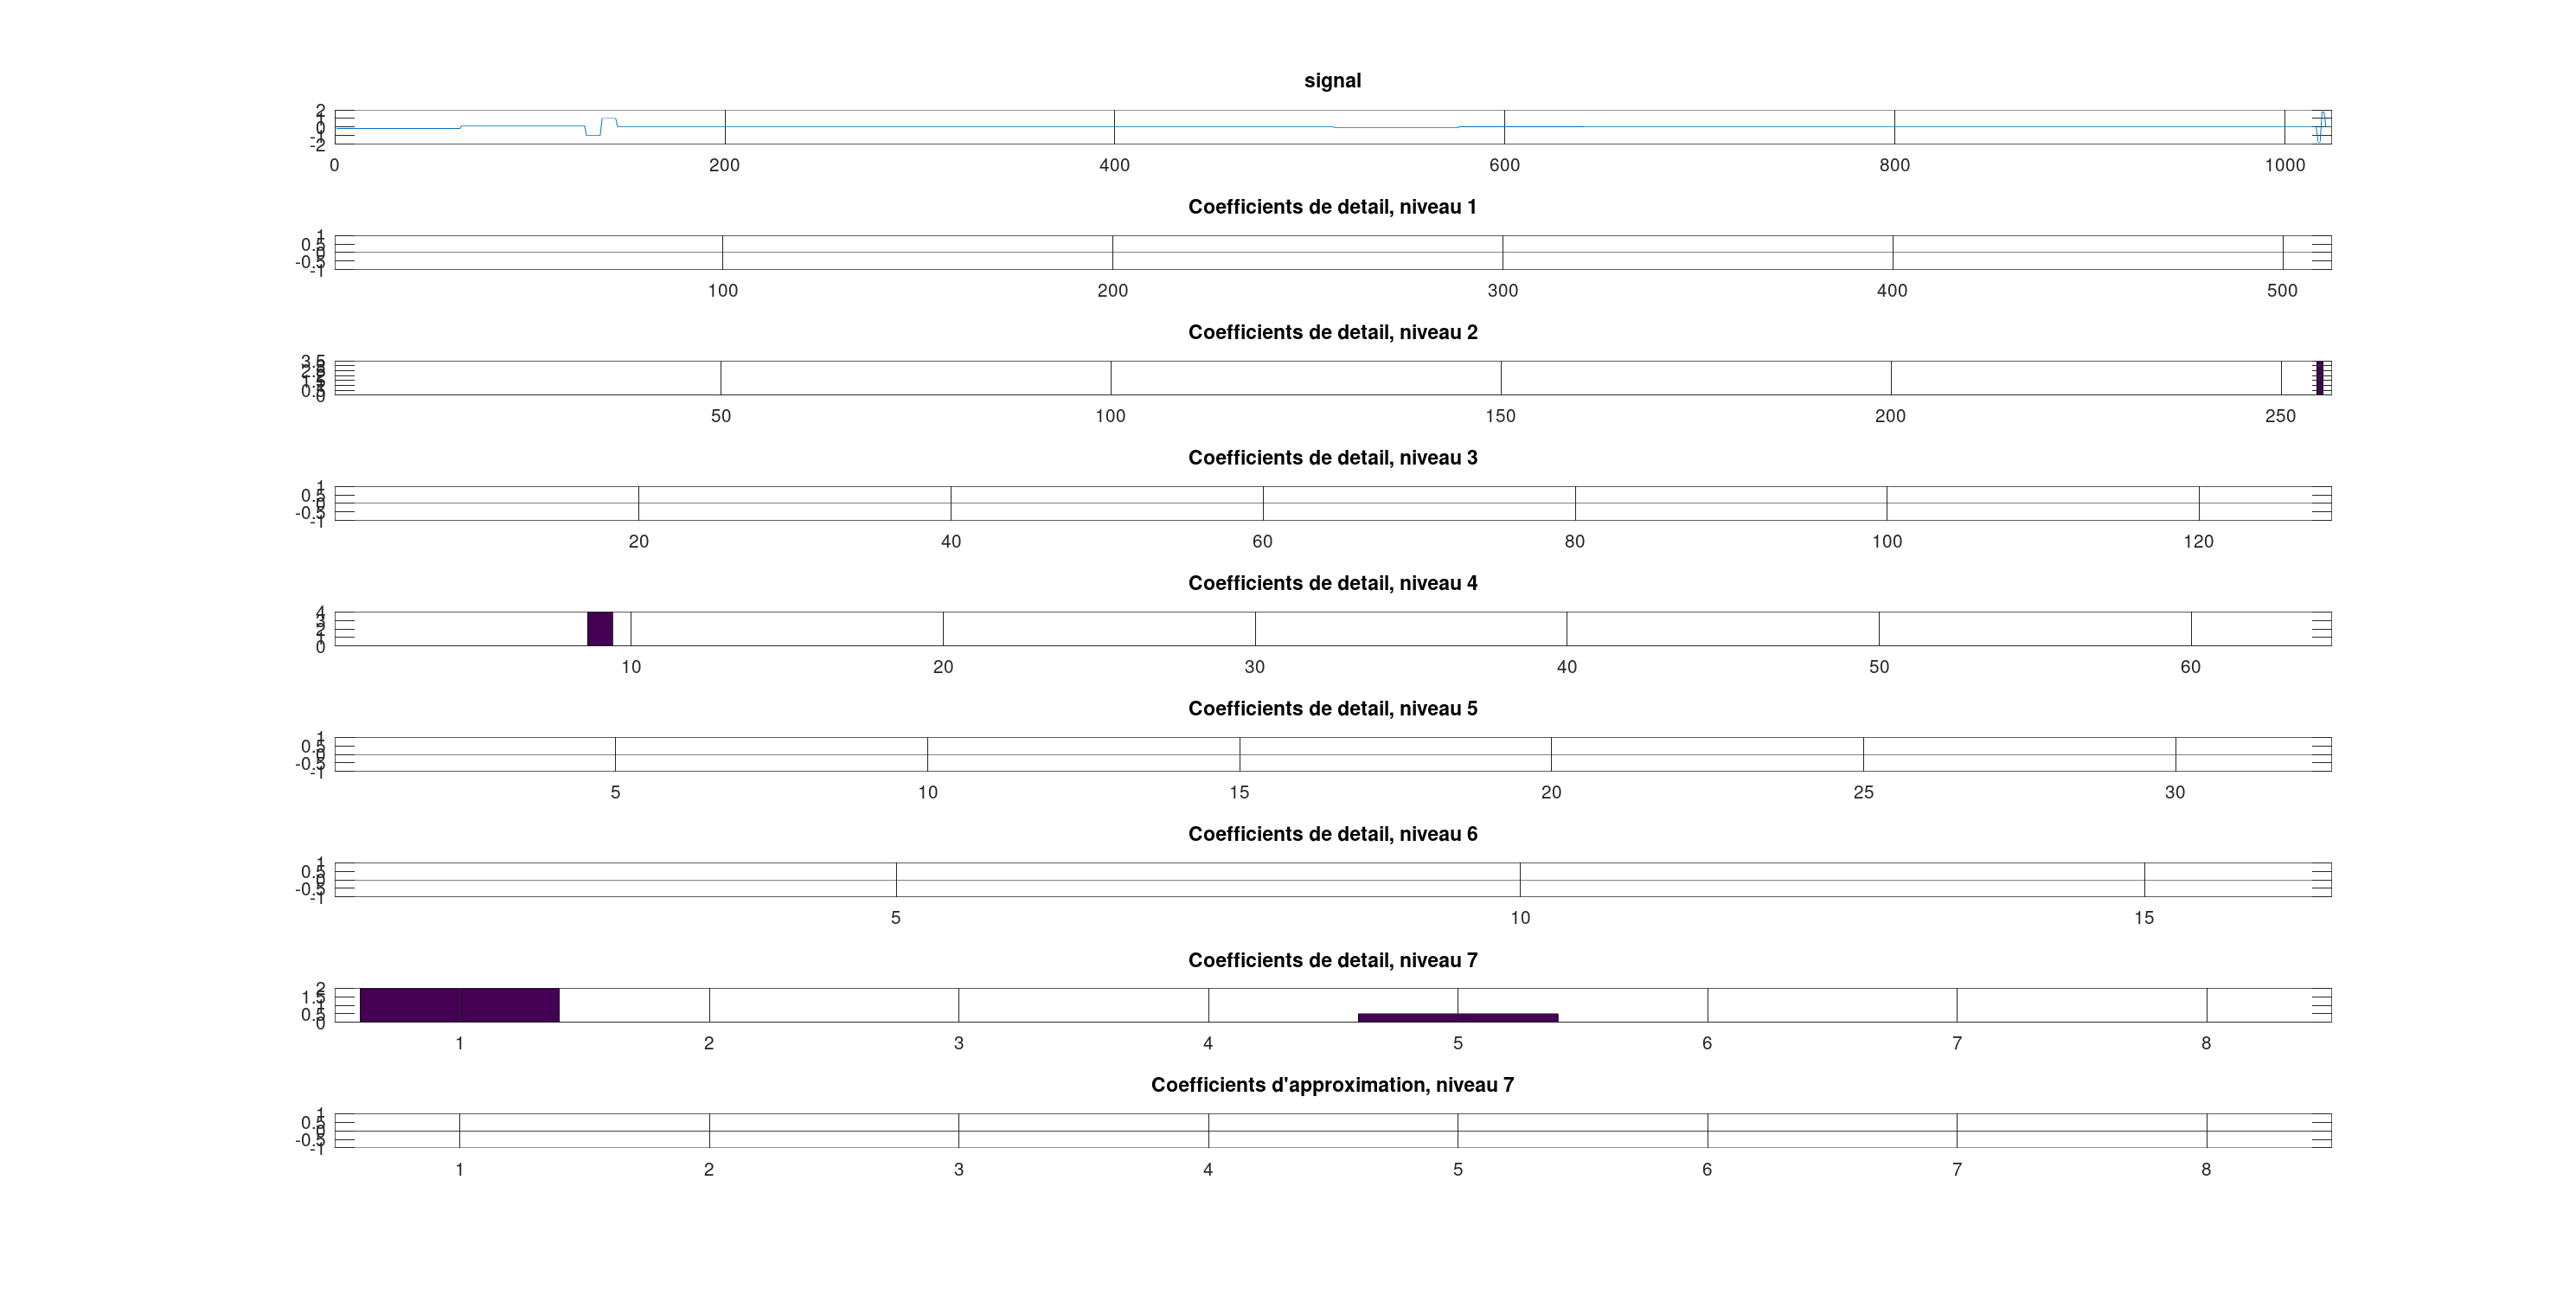
\includegraphics[width=\textwidth]{ex2_1}
                    \centering
                \end{figure}
            }

        \item{Ajoutons du bruit au signal obtenu et visualisons ce nouveau
                signal ainsi que sa FWT :

                \begin{figure}[H]
                    \caption{Signal bruité et sa DWT}
                    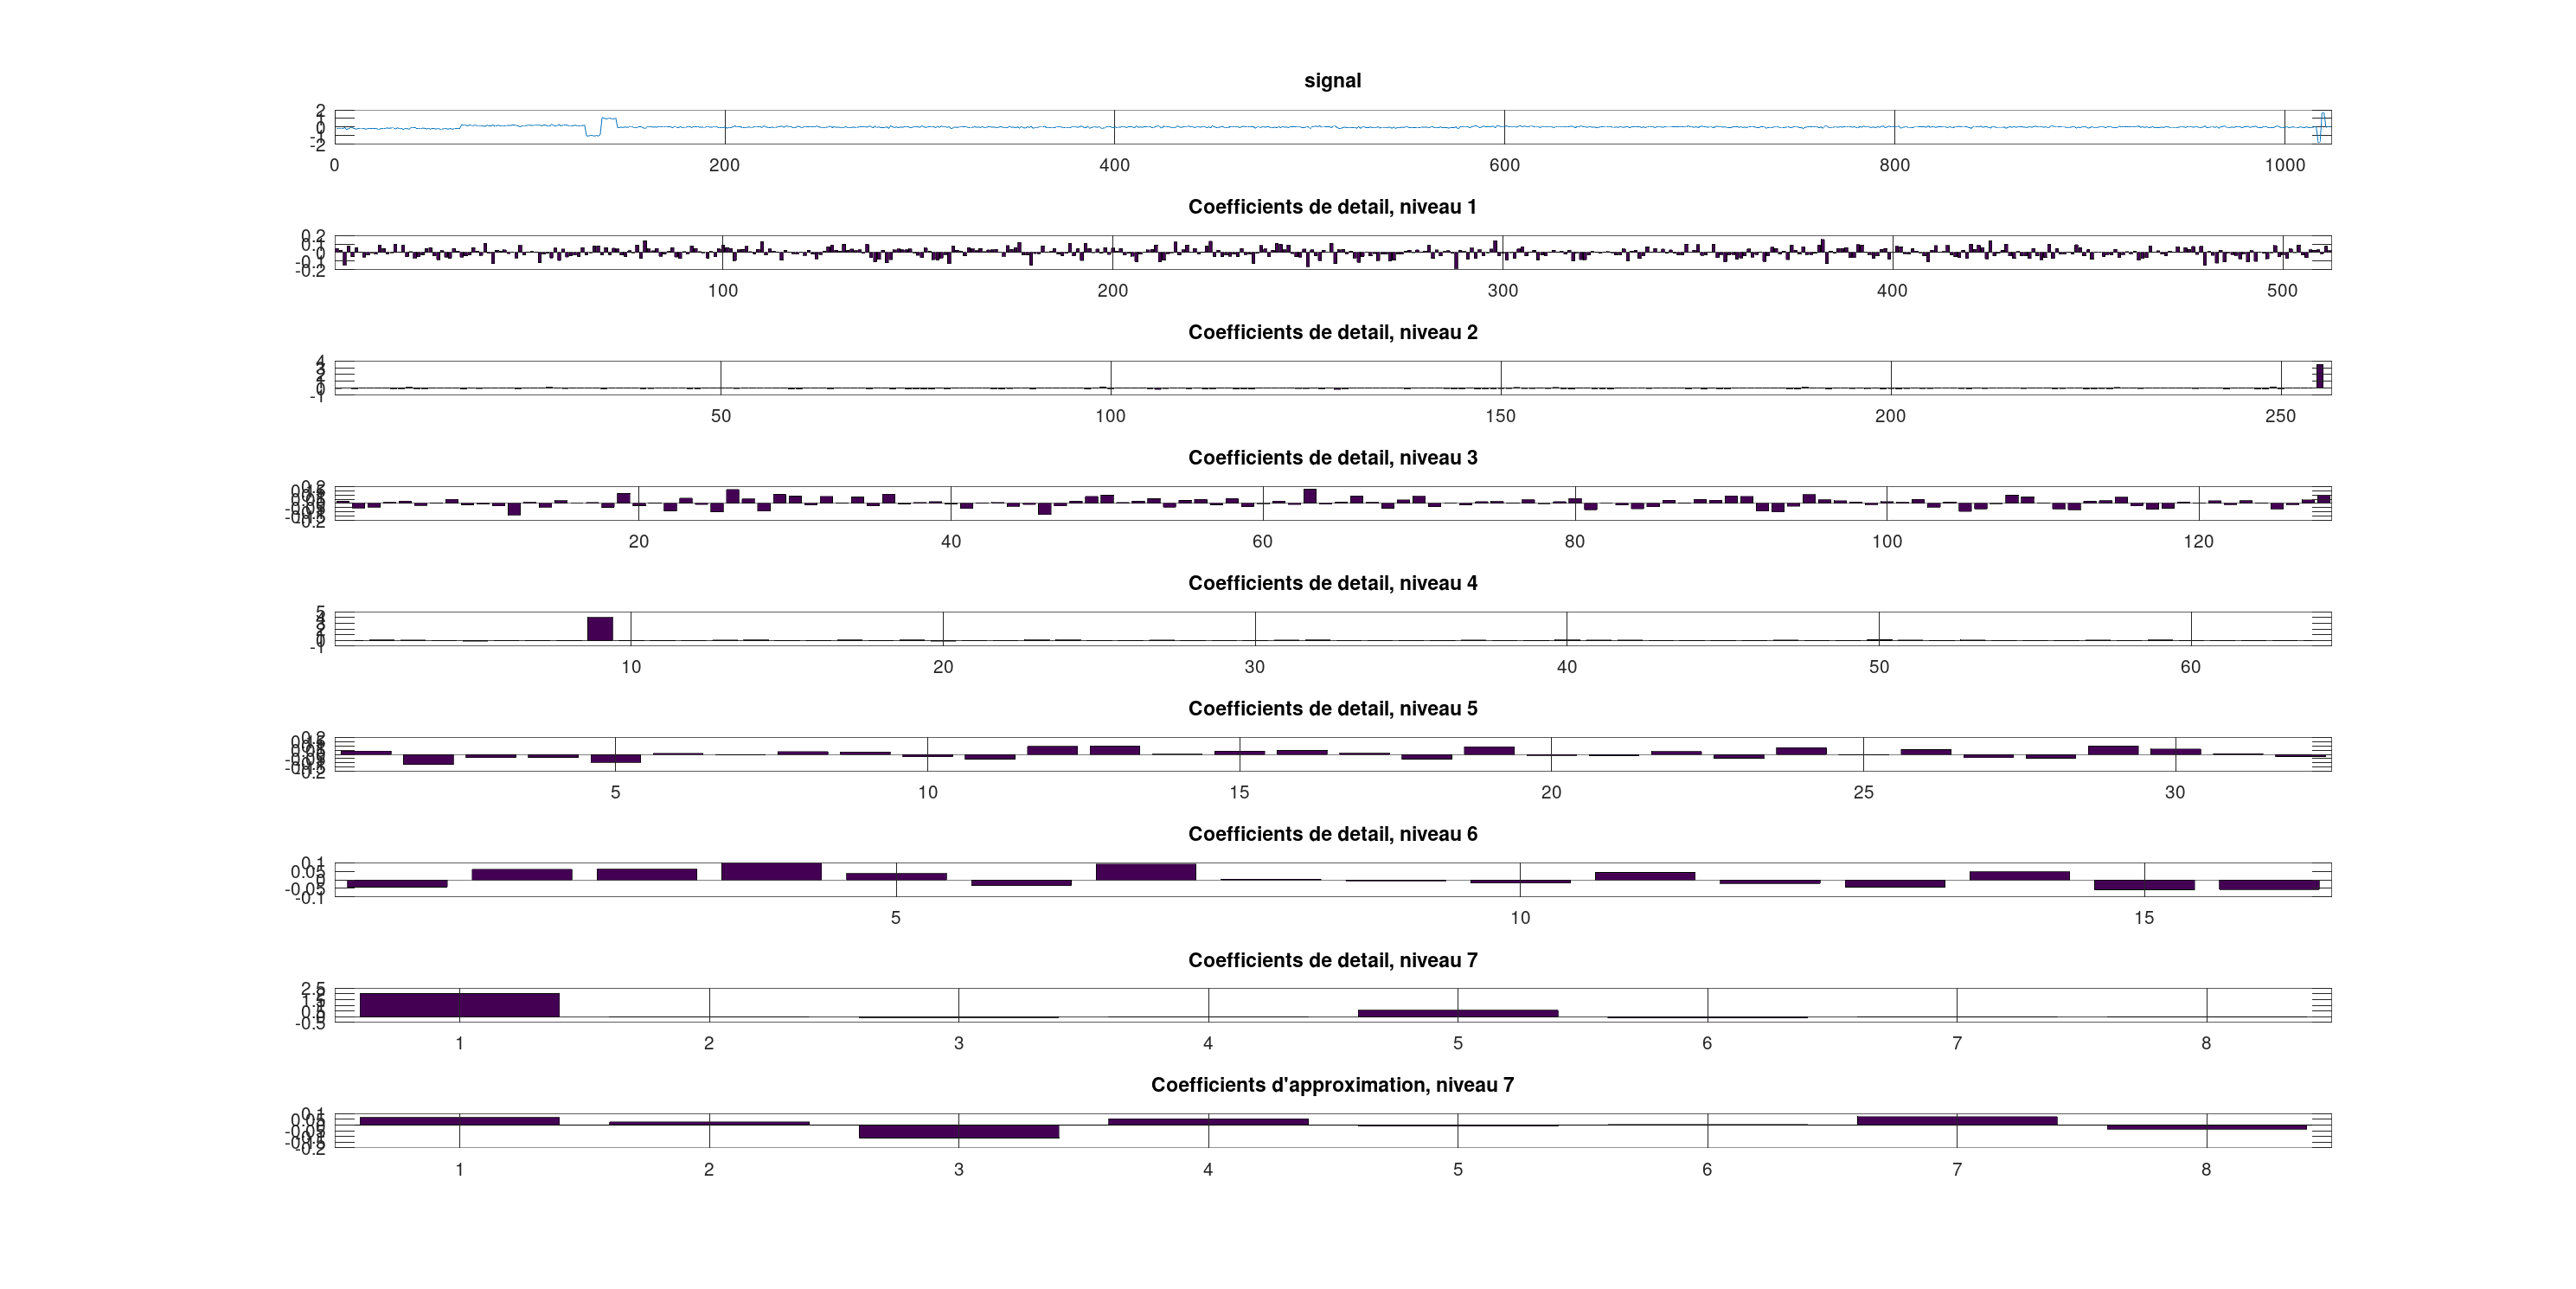
\includegraphics[width=\textwidth]{ex2_2}
                    \centering
                \end{figure}

                On observe ainsi que l'ajout de bruit au signal résulte
                également en un ajout de bruit à sa DWT. Toutefois on
                remarque que les nouveaux coefficients non nuls liés au
                bruit sont d'amplitude faible devant celle des coefficients
                de la DWT du signal sans bruit.Un filtrage des coefficients
                à l'aide d'un seuil devrait permettre un débruitage du signal.
            }

        \item{Mettons maintenant en œuvre le processus de débruitage décrit.
                Représentons alors l'erreur de construction commise en fonction
                de la valeur du seuil $\alpha$ et celle correspondant au seuil
                $\alpha^* = \sigma_b \sqrt{2 ln(N)}$ :

                \begin{figure}[H]
                    \caption{Erreur de reconstruction en fonction de alpha}
                    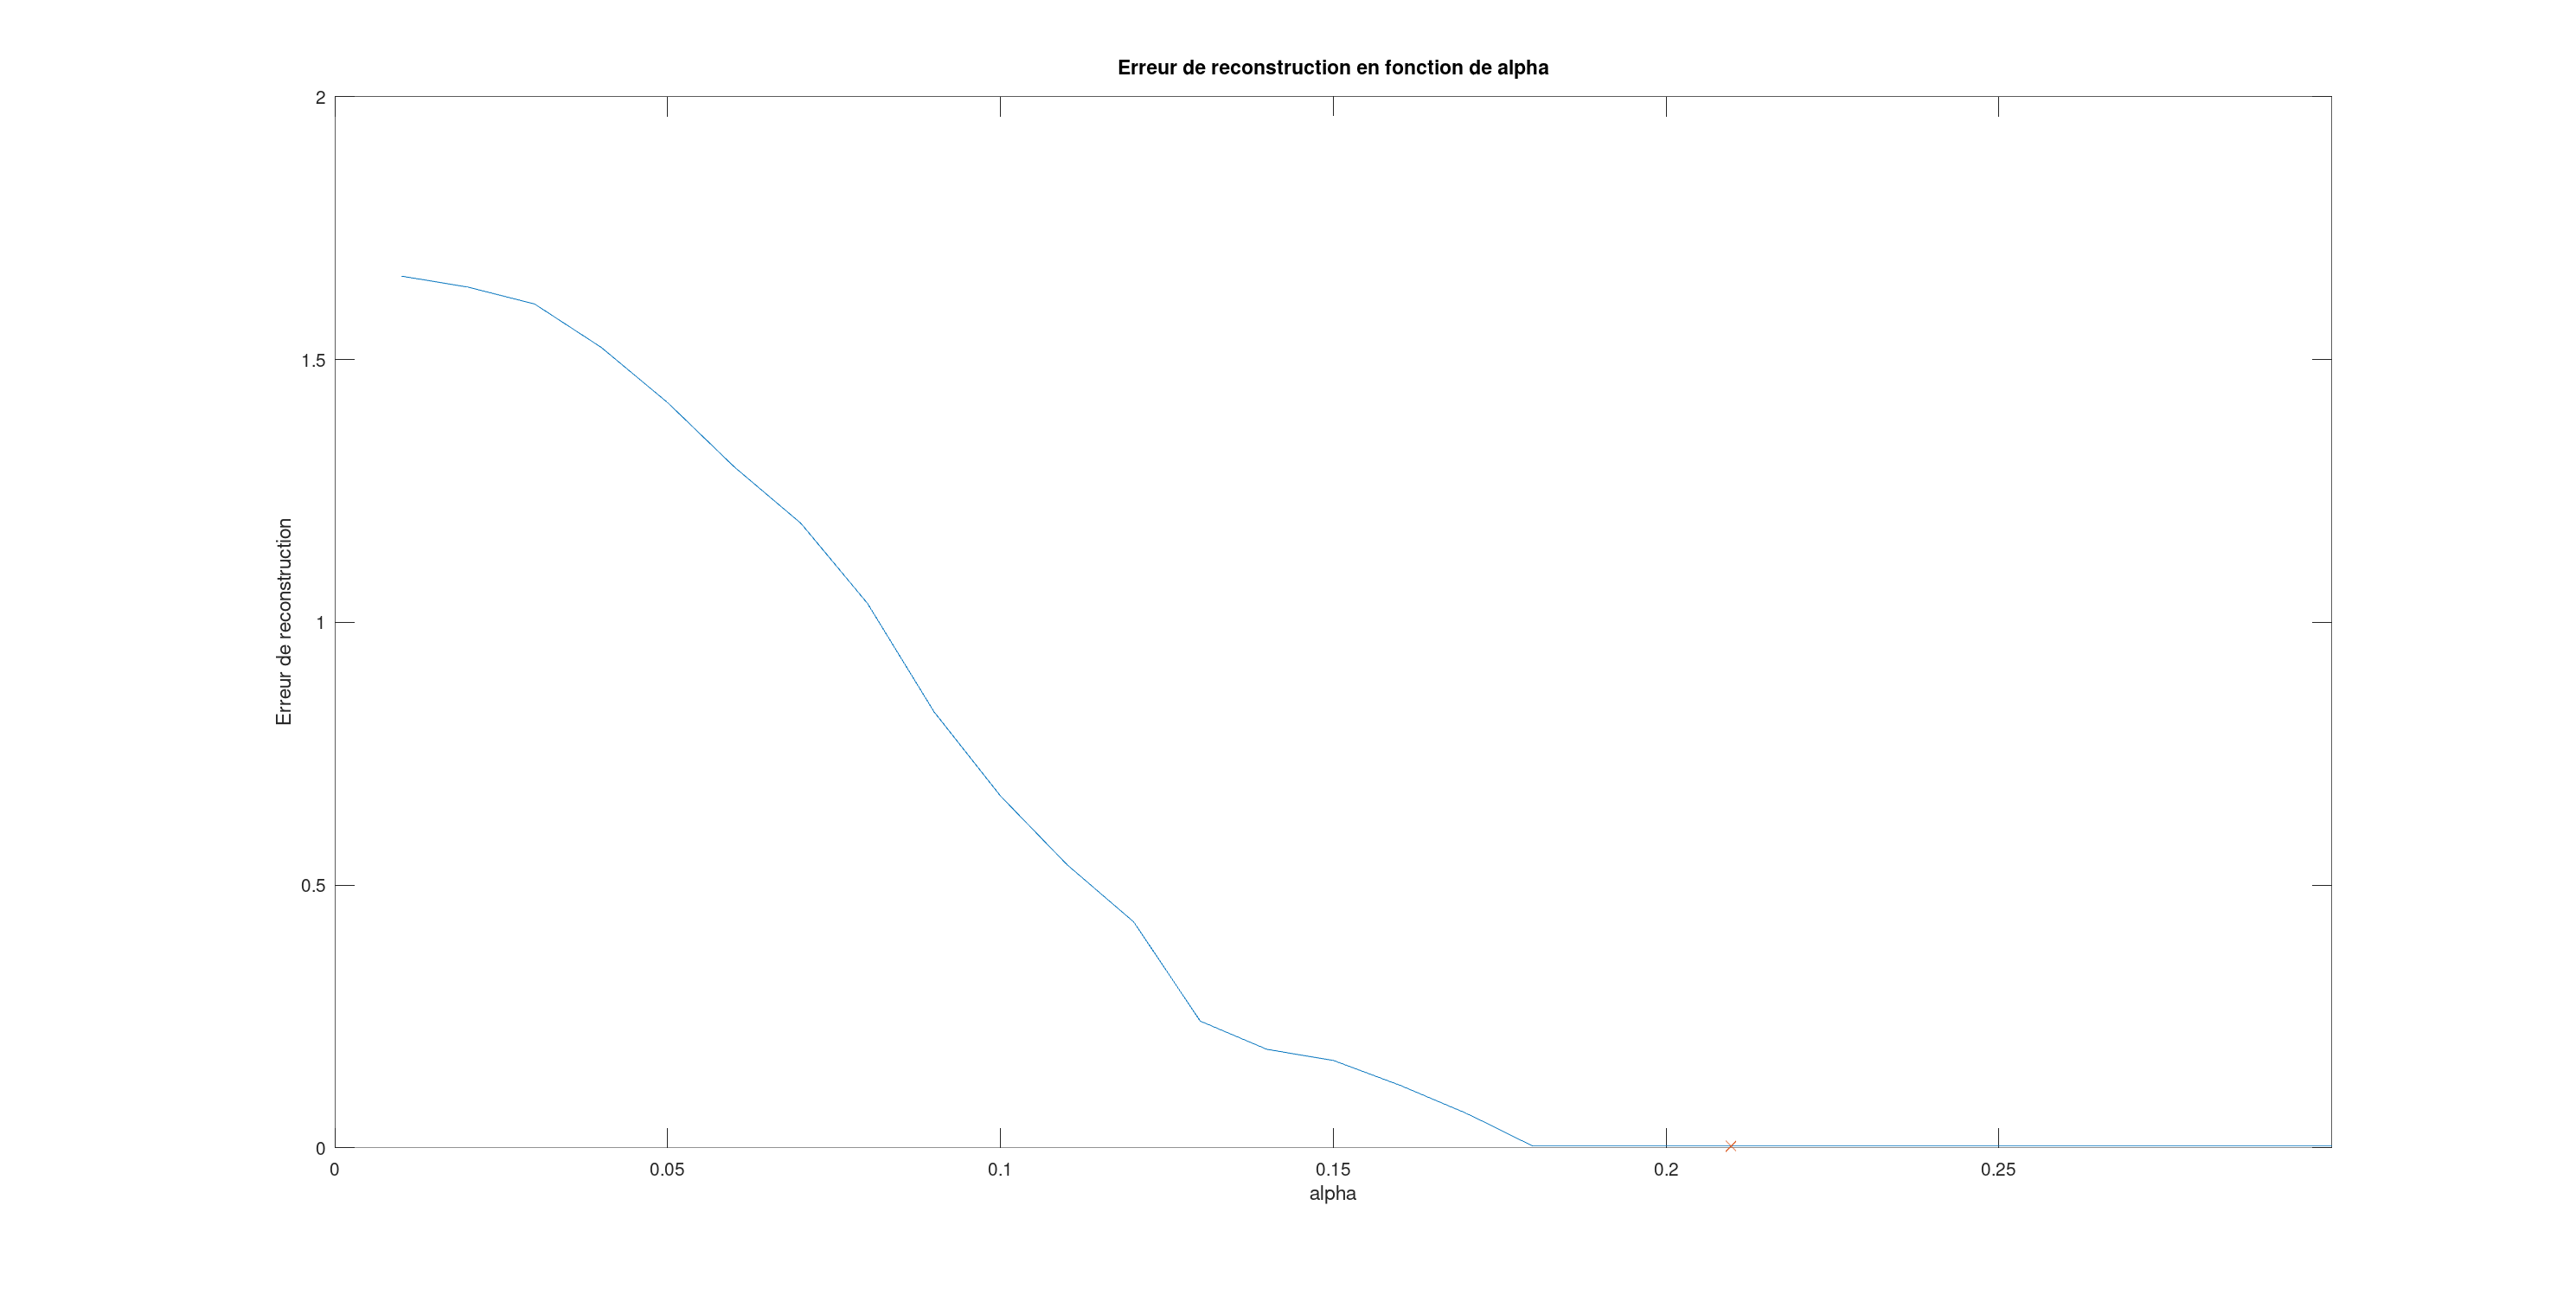
\includegraphics[width=\textwidth]{ex2_3}
                    \centering
                \end{figure}
            }

        \item{On génère les signaux "Blocks" et "Doppler" à l'aide de la
            fonction \texttt{makesig}.}

        \item{Représentons ces deux signaux ainsi que leur DWT :

                \begin{figure}[H]
                    \caption{Singal "Blocks" et sa DWT}
                    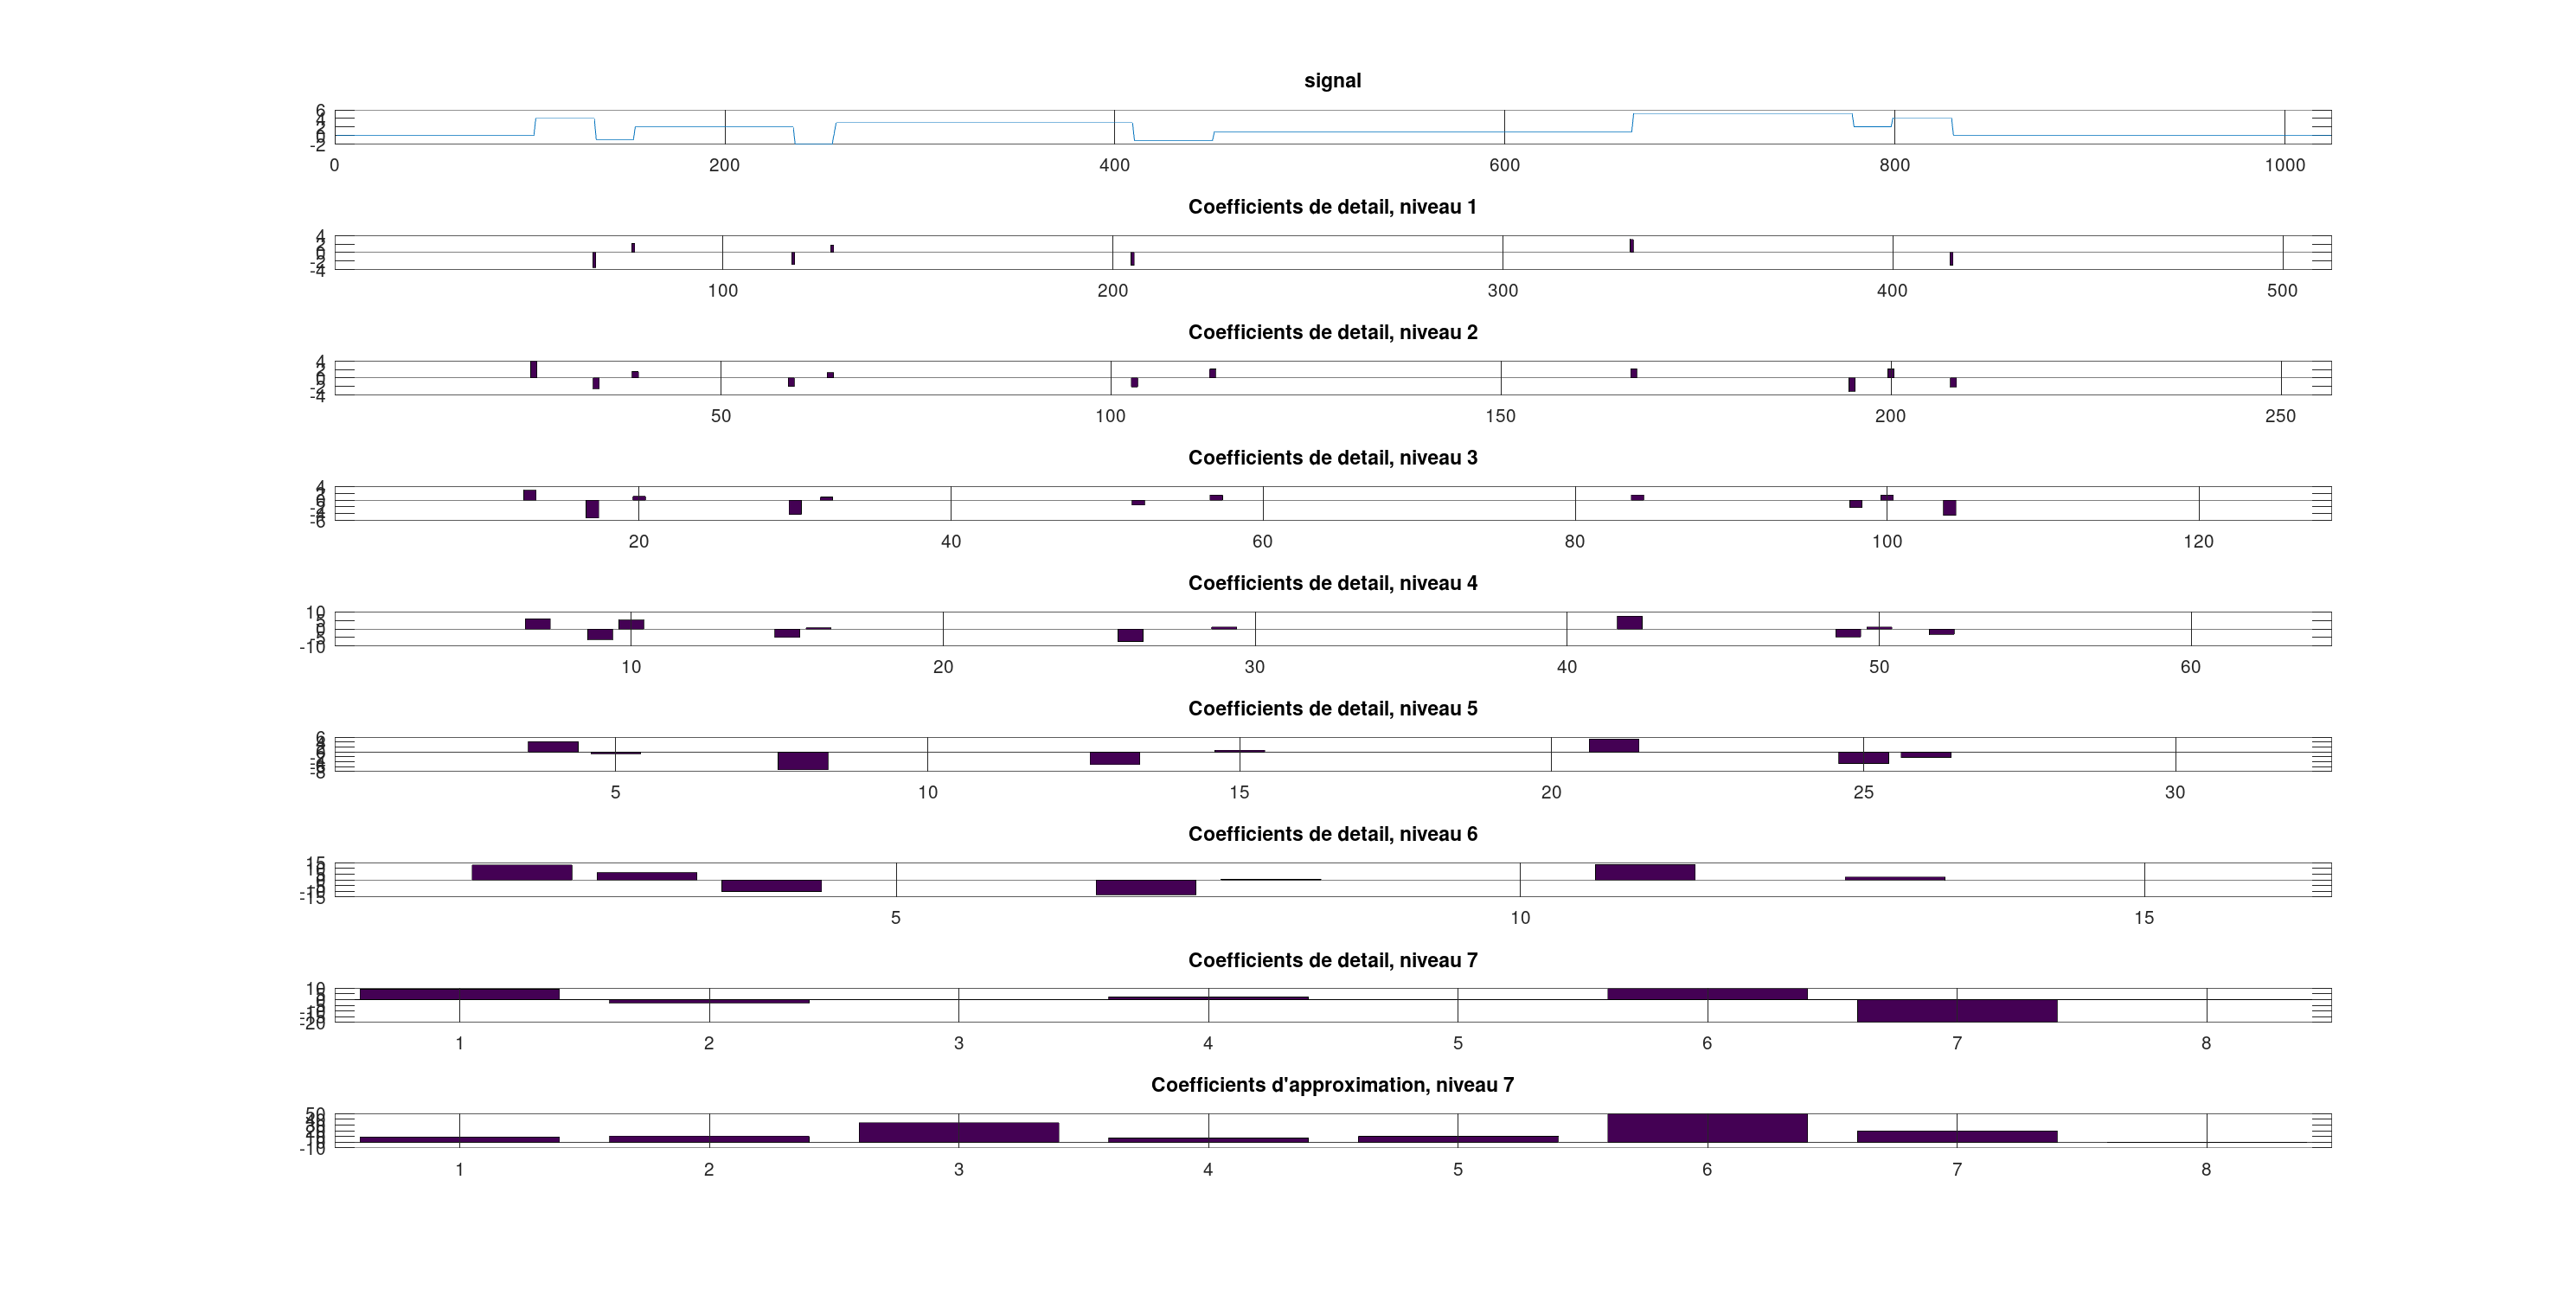
\includegraphics[width=\textwidth]{ex2_4}
                    \centering
                \end{figure}

                \begin{figure}[H]
                    \caption{Signal "Dopler" et sa DWT}
                    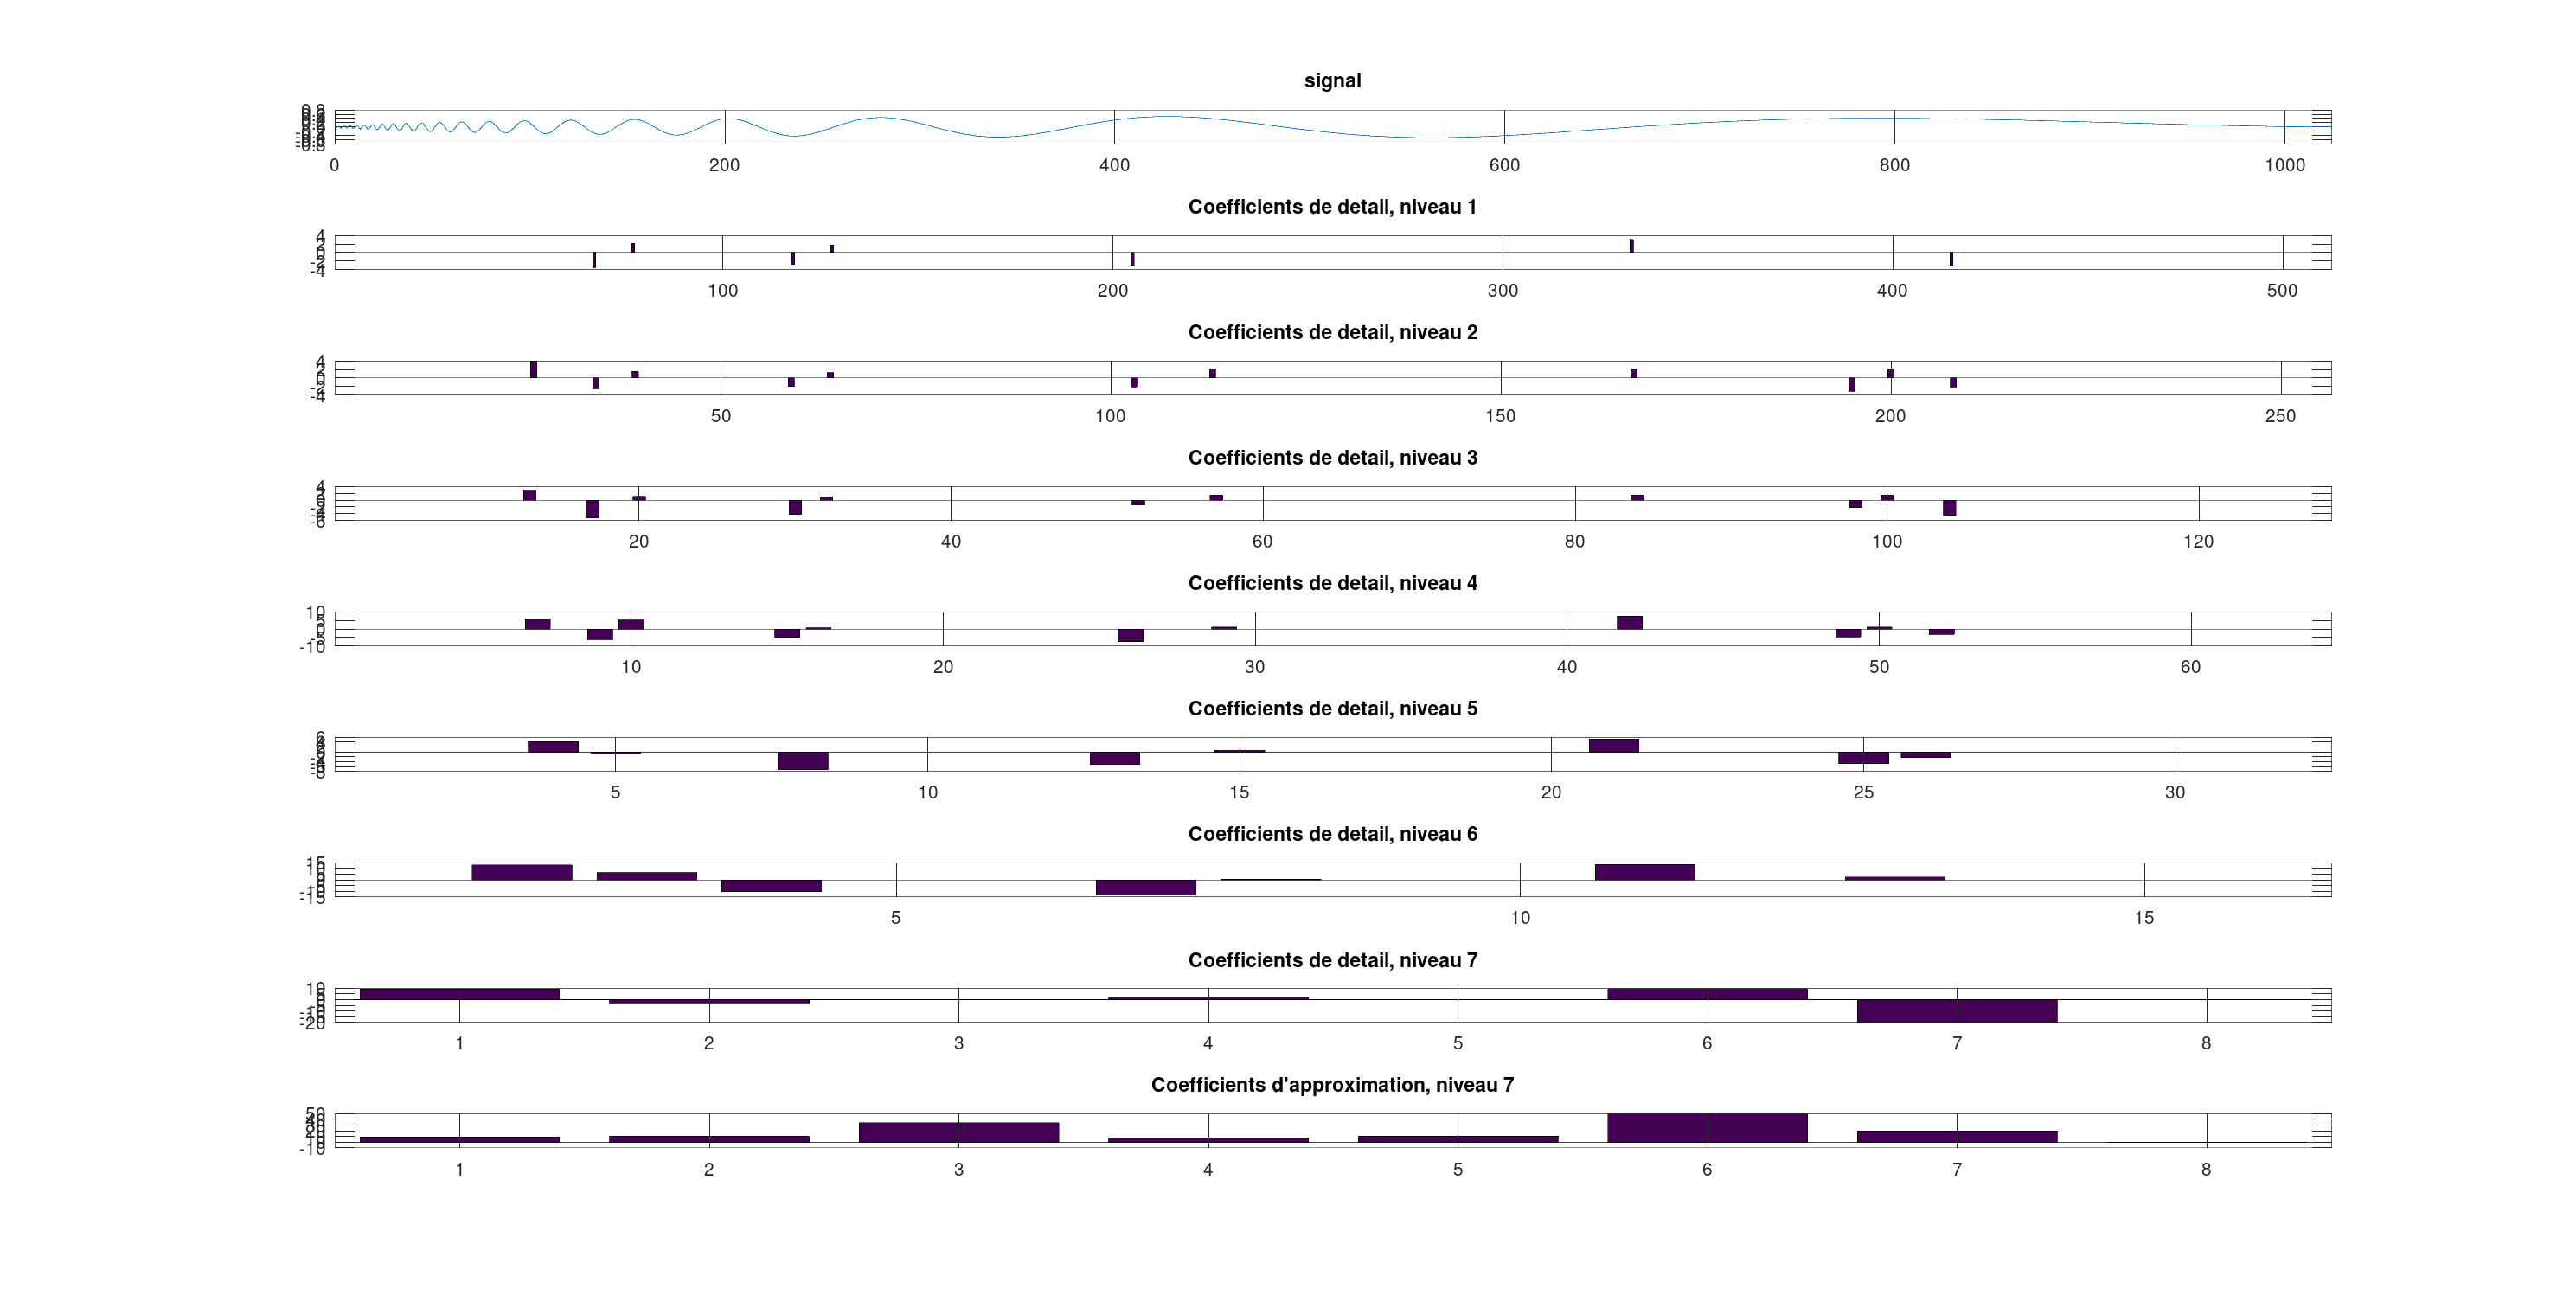
\includegraphics[width=\textwidth]{ex2_5}
                    \centering
                \end{figure}

                Ajoutons du bruit avec un RSD de 20 dB et appliquons la
                procédure précédente. On obtient les tracés d'erreur de
                reconstruction en fonction du seuil suivants :

                \begin{figure}[H]
                    \caption{Erreur de reconstruction en fonction du bruit (Blocks)}
                    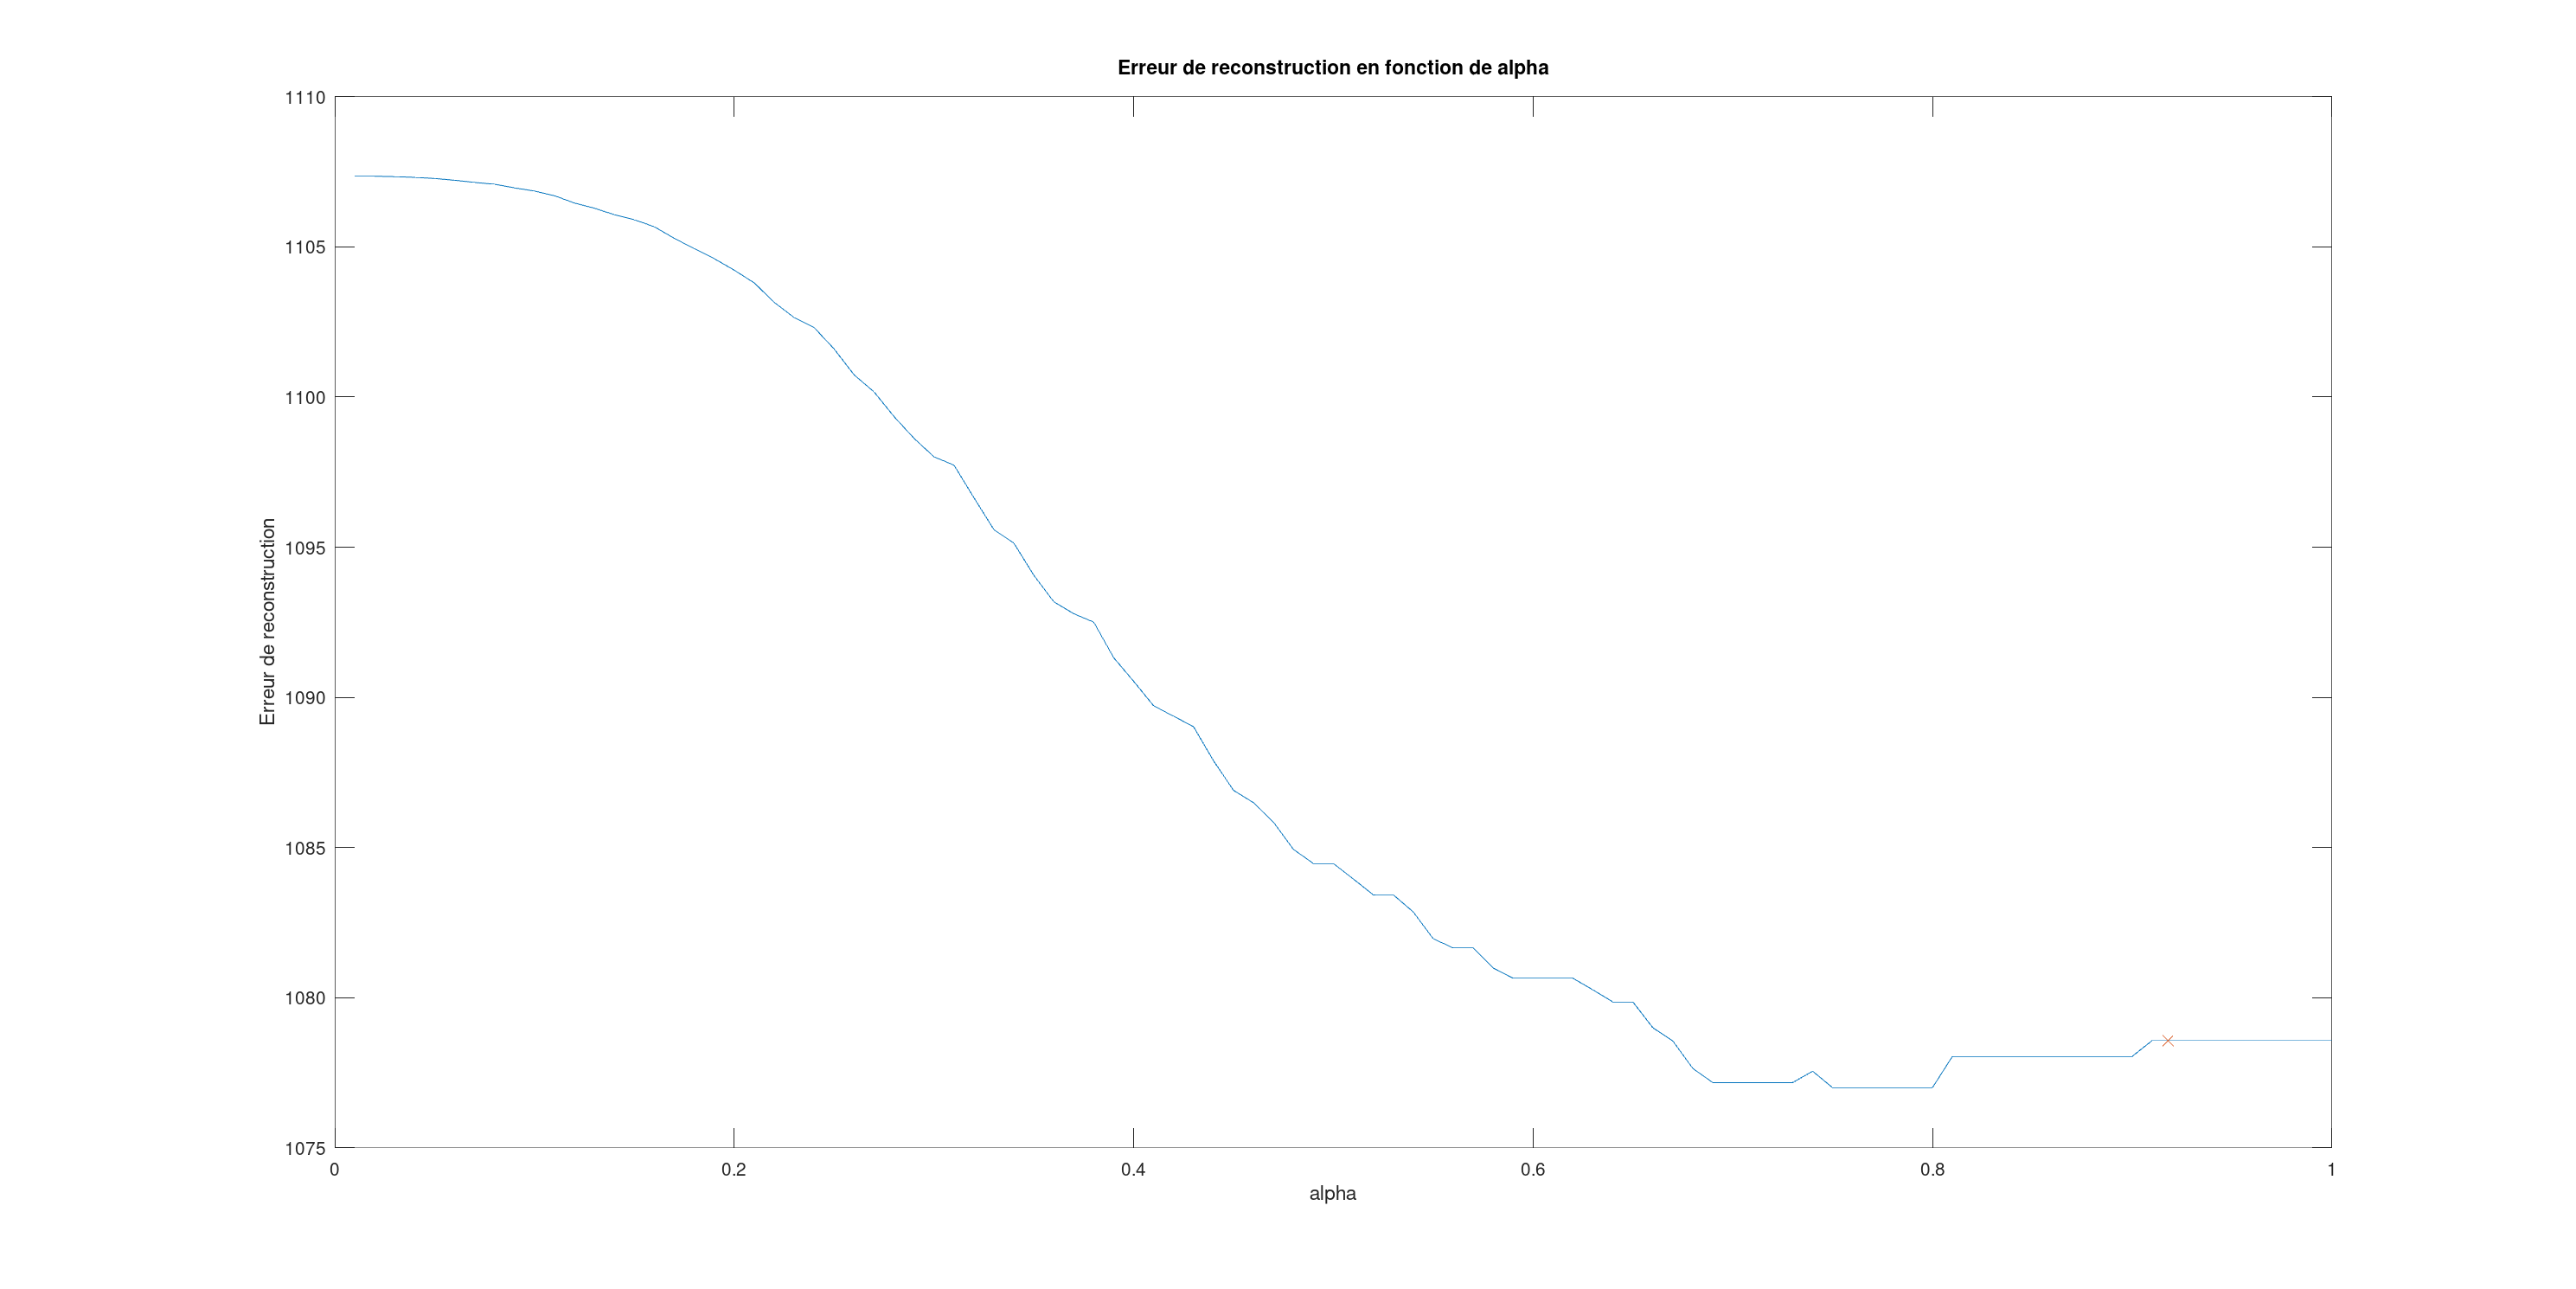
\includegraphics[width=\textwidth]{ex2_6}
                    \centering
                \end{figure}

                \begin{figure}[H]
                    \caption{Erreur de reconstruction en fonction du bruit (Dopler)}
                    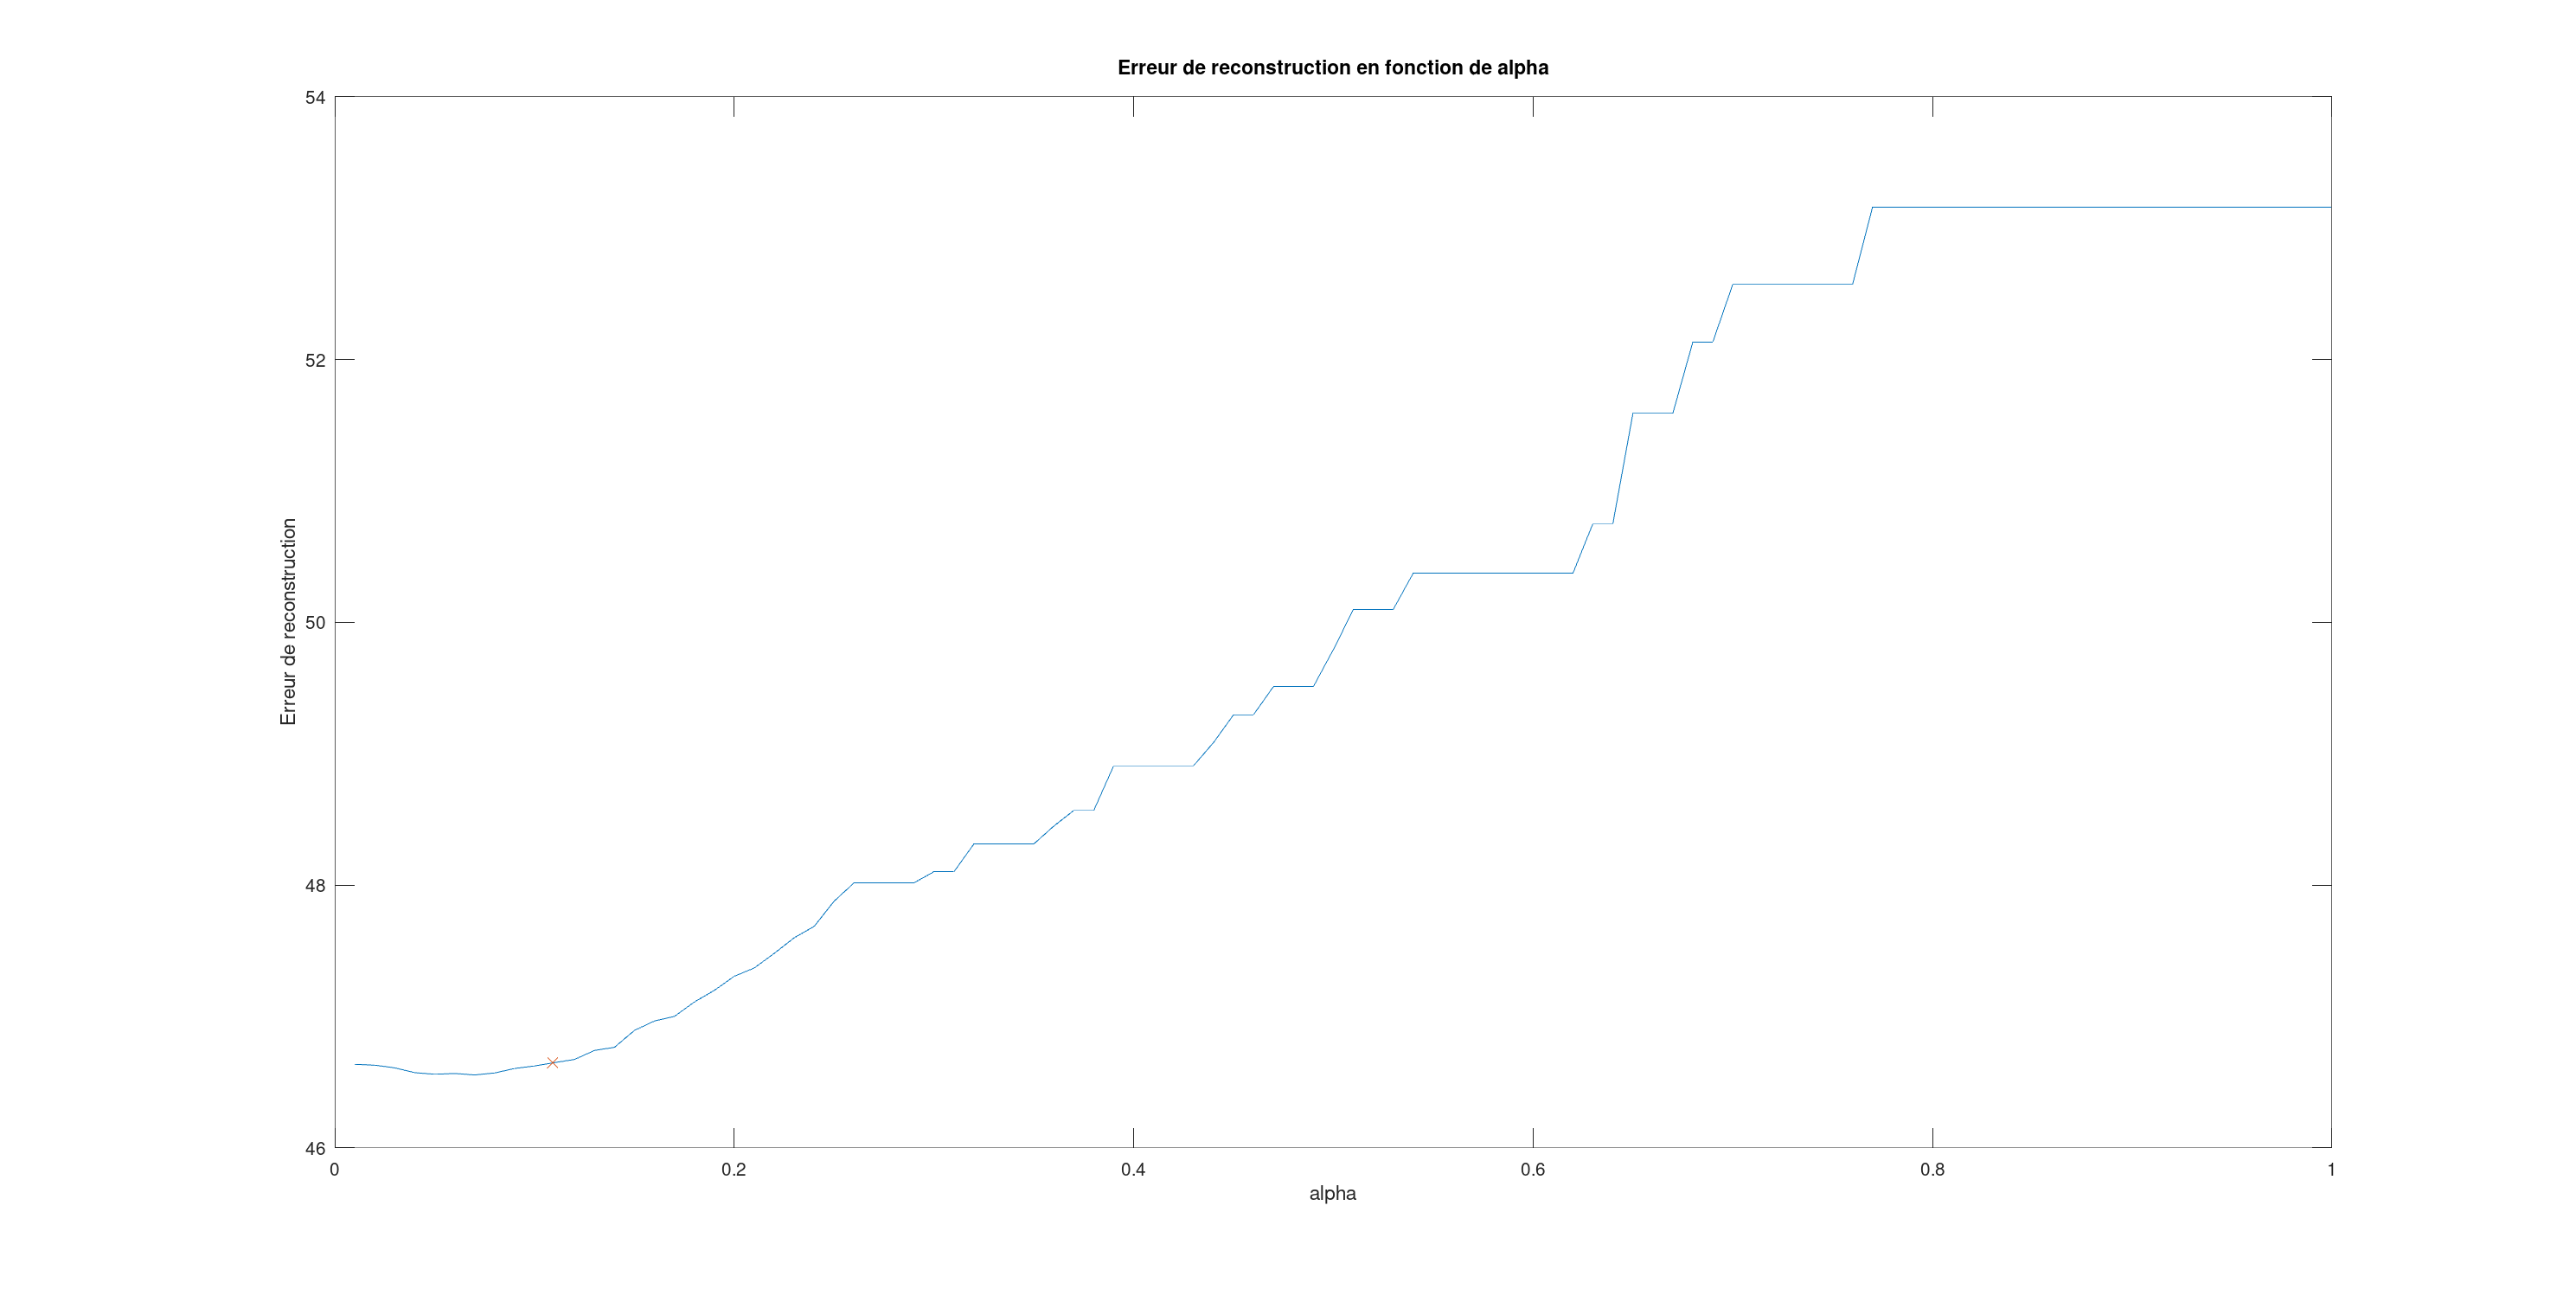
\includegraphics[width=\textwidth]{ex2_7}
                    \centering
                \end{figure}
            }

        \item{En utilisant maintenant une ondelette de Daubechies d'ordre 4,
                on obtient les tracés suivants :

                \begin{figure}[H]
                    \caption{Erreur de reconstruction en fonction du bruit (Blocks)}
                    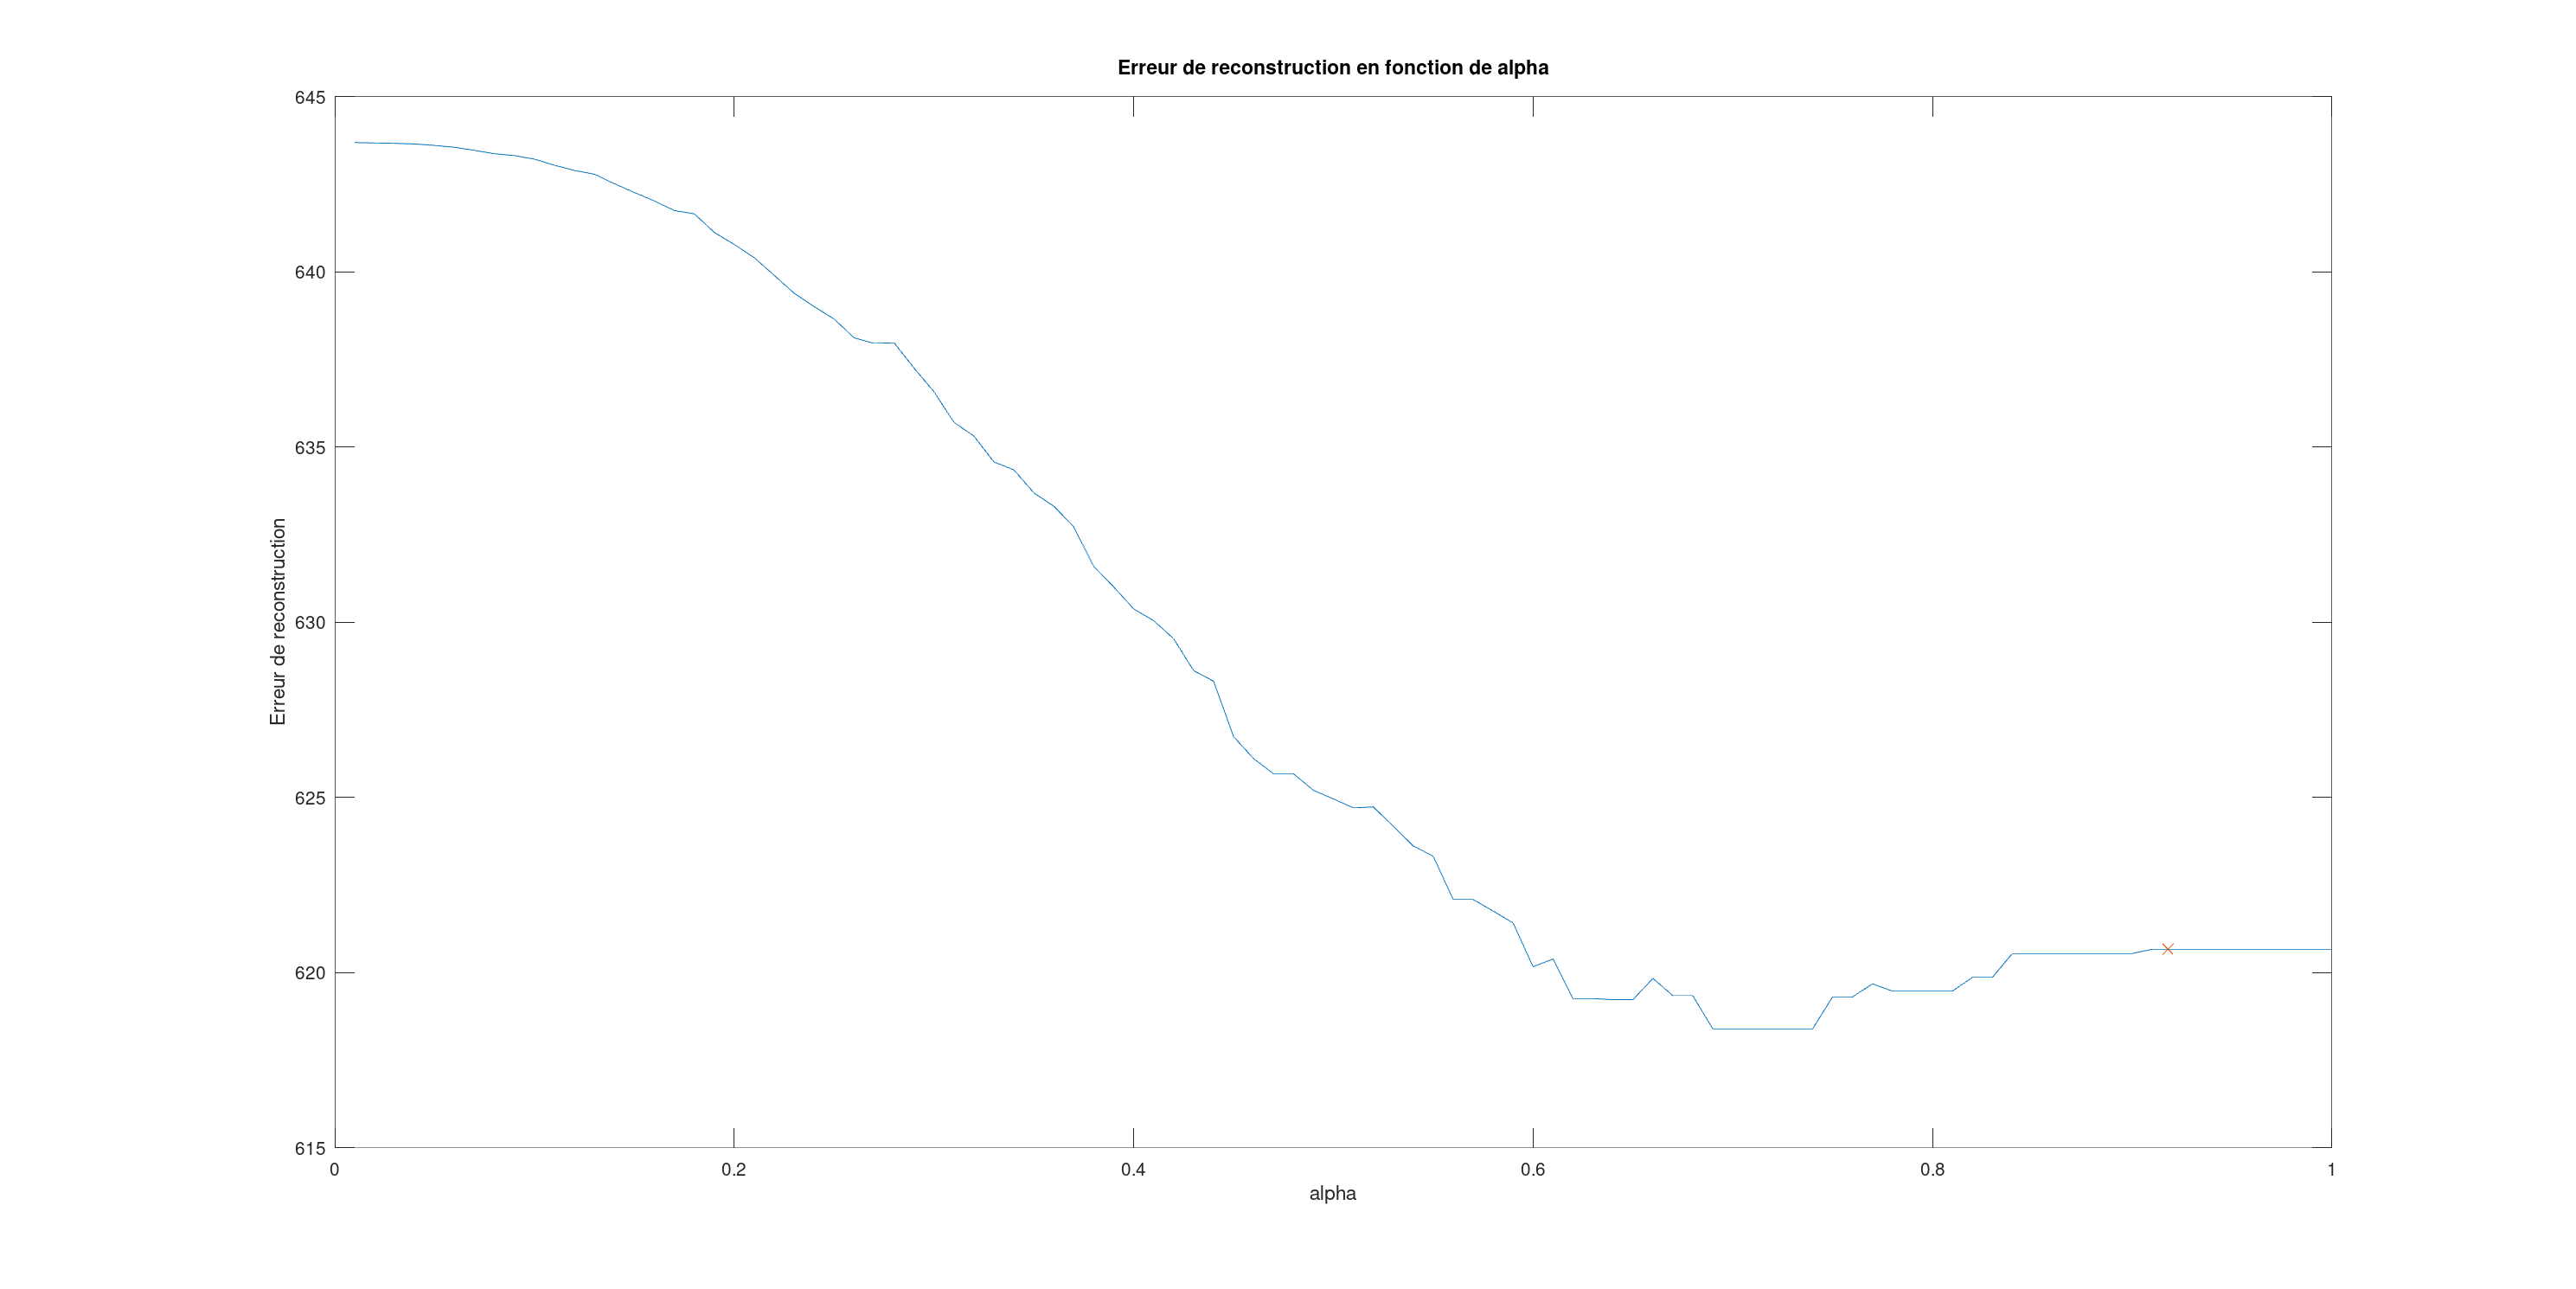
\includegraphics[width=\textwidth]{ex2_6bis}
                    \centering
                \end{figure}

                \begin{figure}[H]
                    \caption{Erreur de reconstruction en fonction du bruit (Dopler)}
                    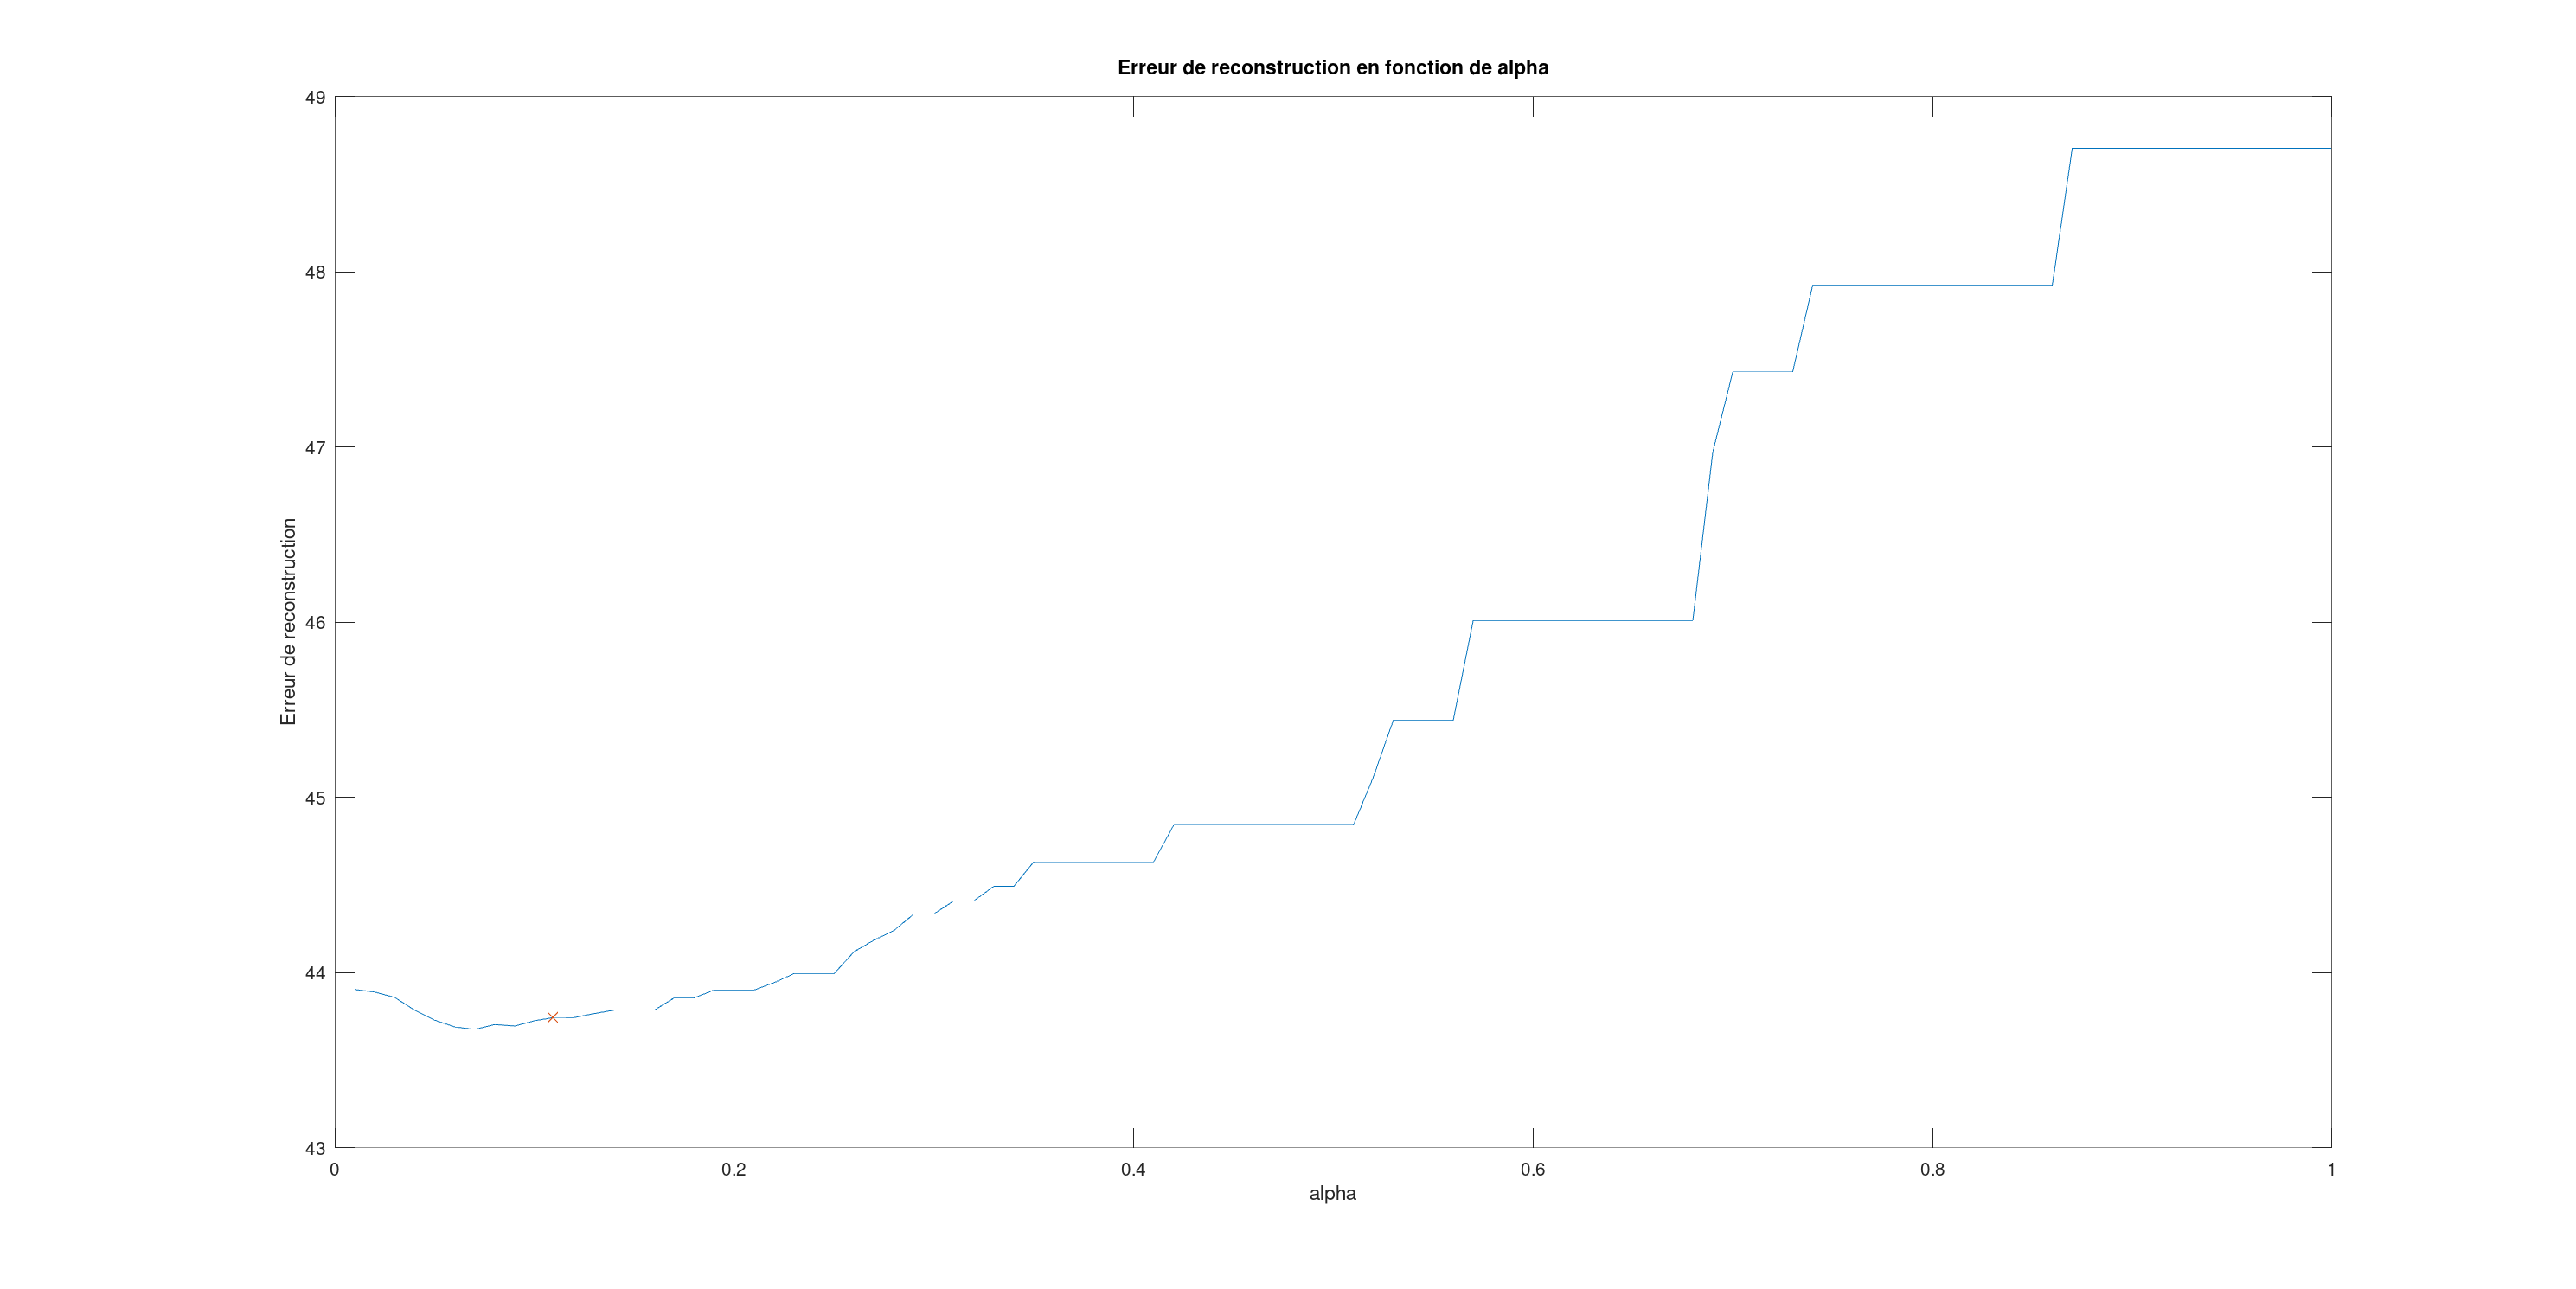
\includegraphics[width=\textwidth]{ex2_7bis}
                    \centering
                \end{figure}

            }

    \end{enumerate}

    \section{Compression d'images}

    \begin{enumerate}

        \item{On ouvre l'image \texttt{peppers.tiff} à l'aide de la fonction
                \texttt{imread} de Matlab.
            }

        \item{
                Visualisions cette image :

                \begin{figure}[H]
                    \caption{Image \texttt{peppers.tiff}}
                    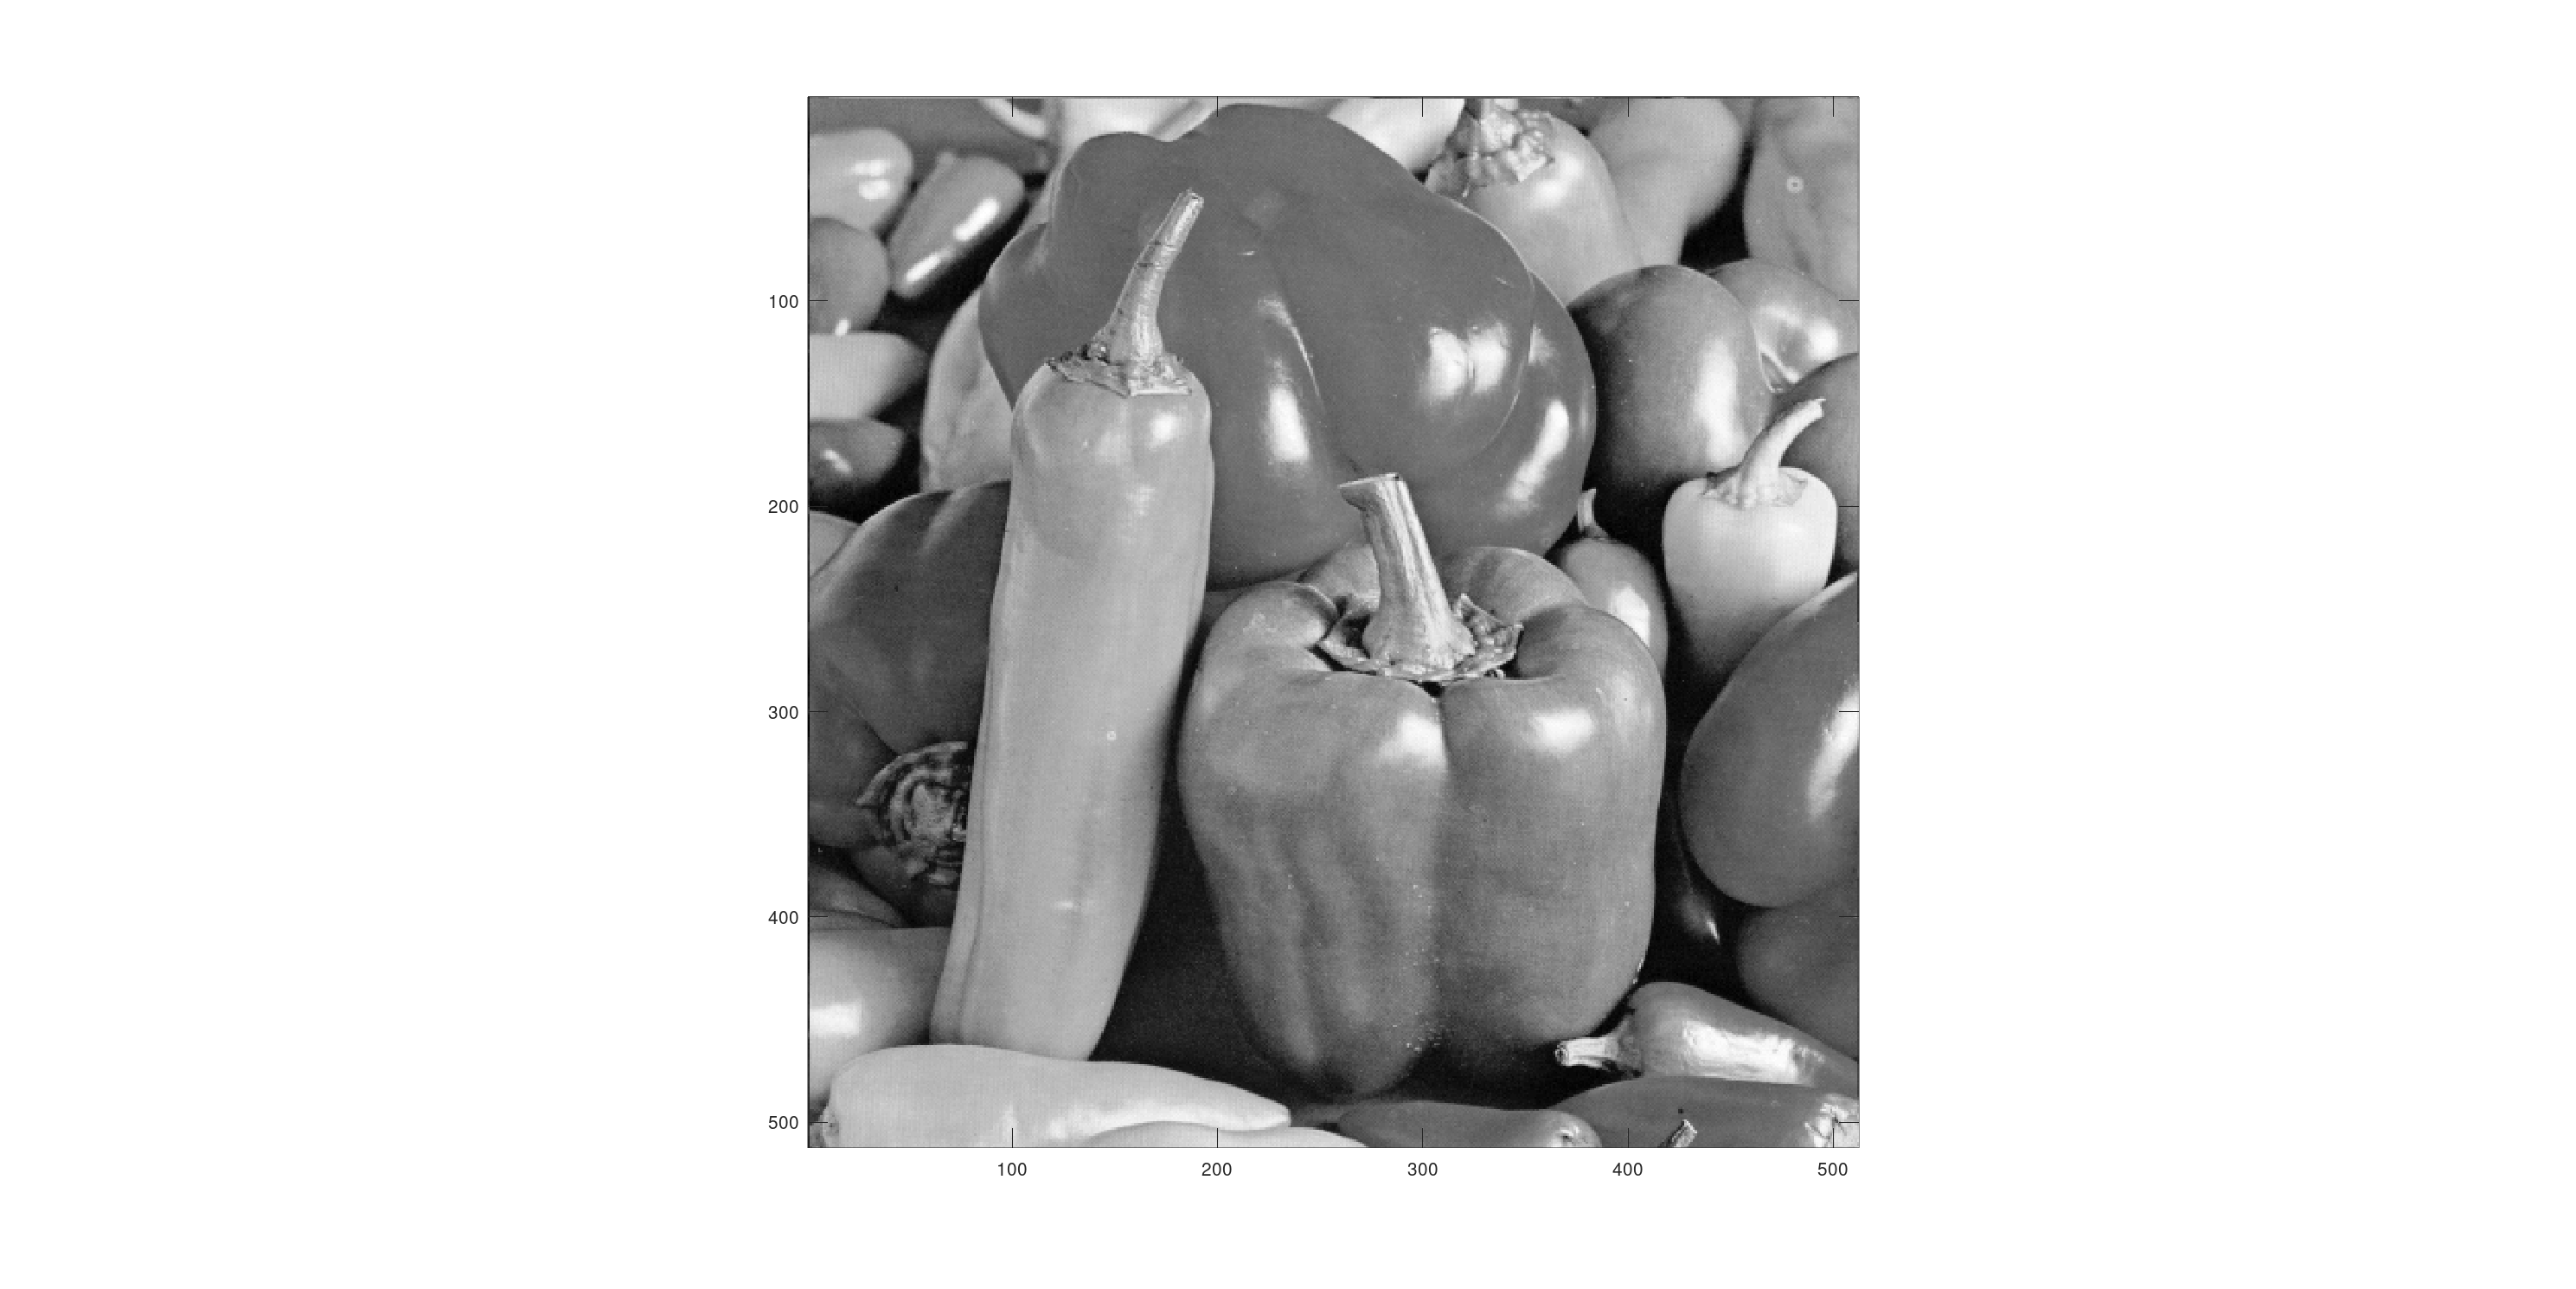
\includegraphics[width=\textwidth]{ex3_1}
                    \centering
                \end{figure}
            }

        \item{On calcule sa transformée en ondelettes 2D à l'échelle J = 4}

        \item{Visualisions alors cette DWT-2D :

                \begin{figure}[H]
                    \caption{DWT-2D}
                    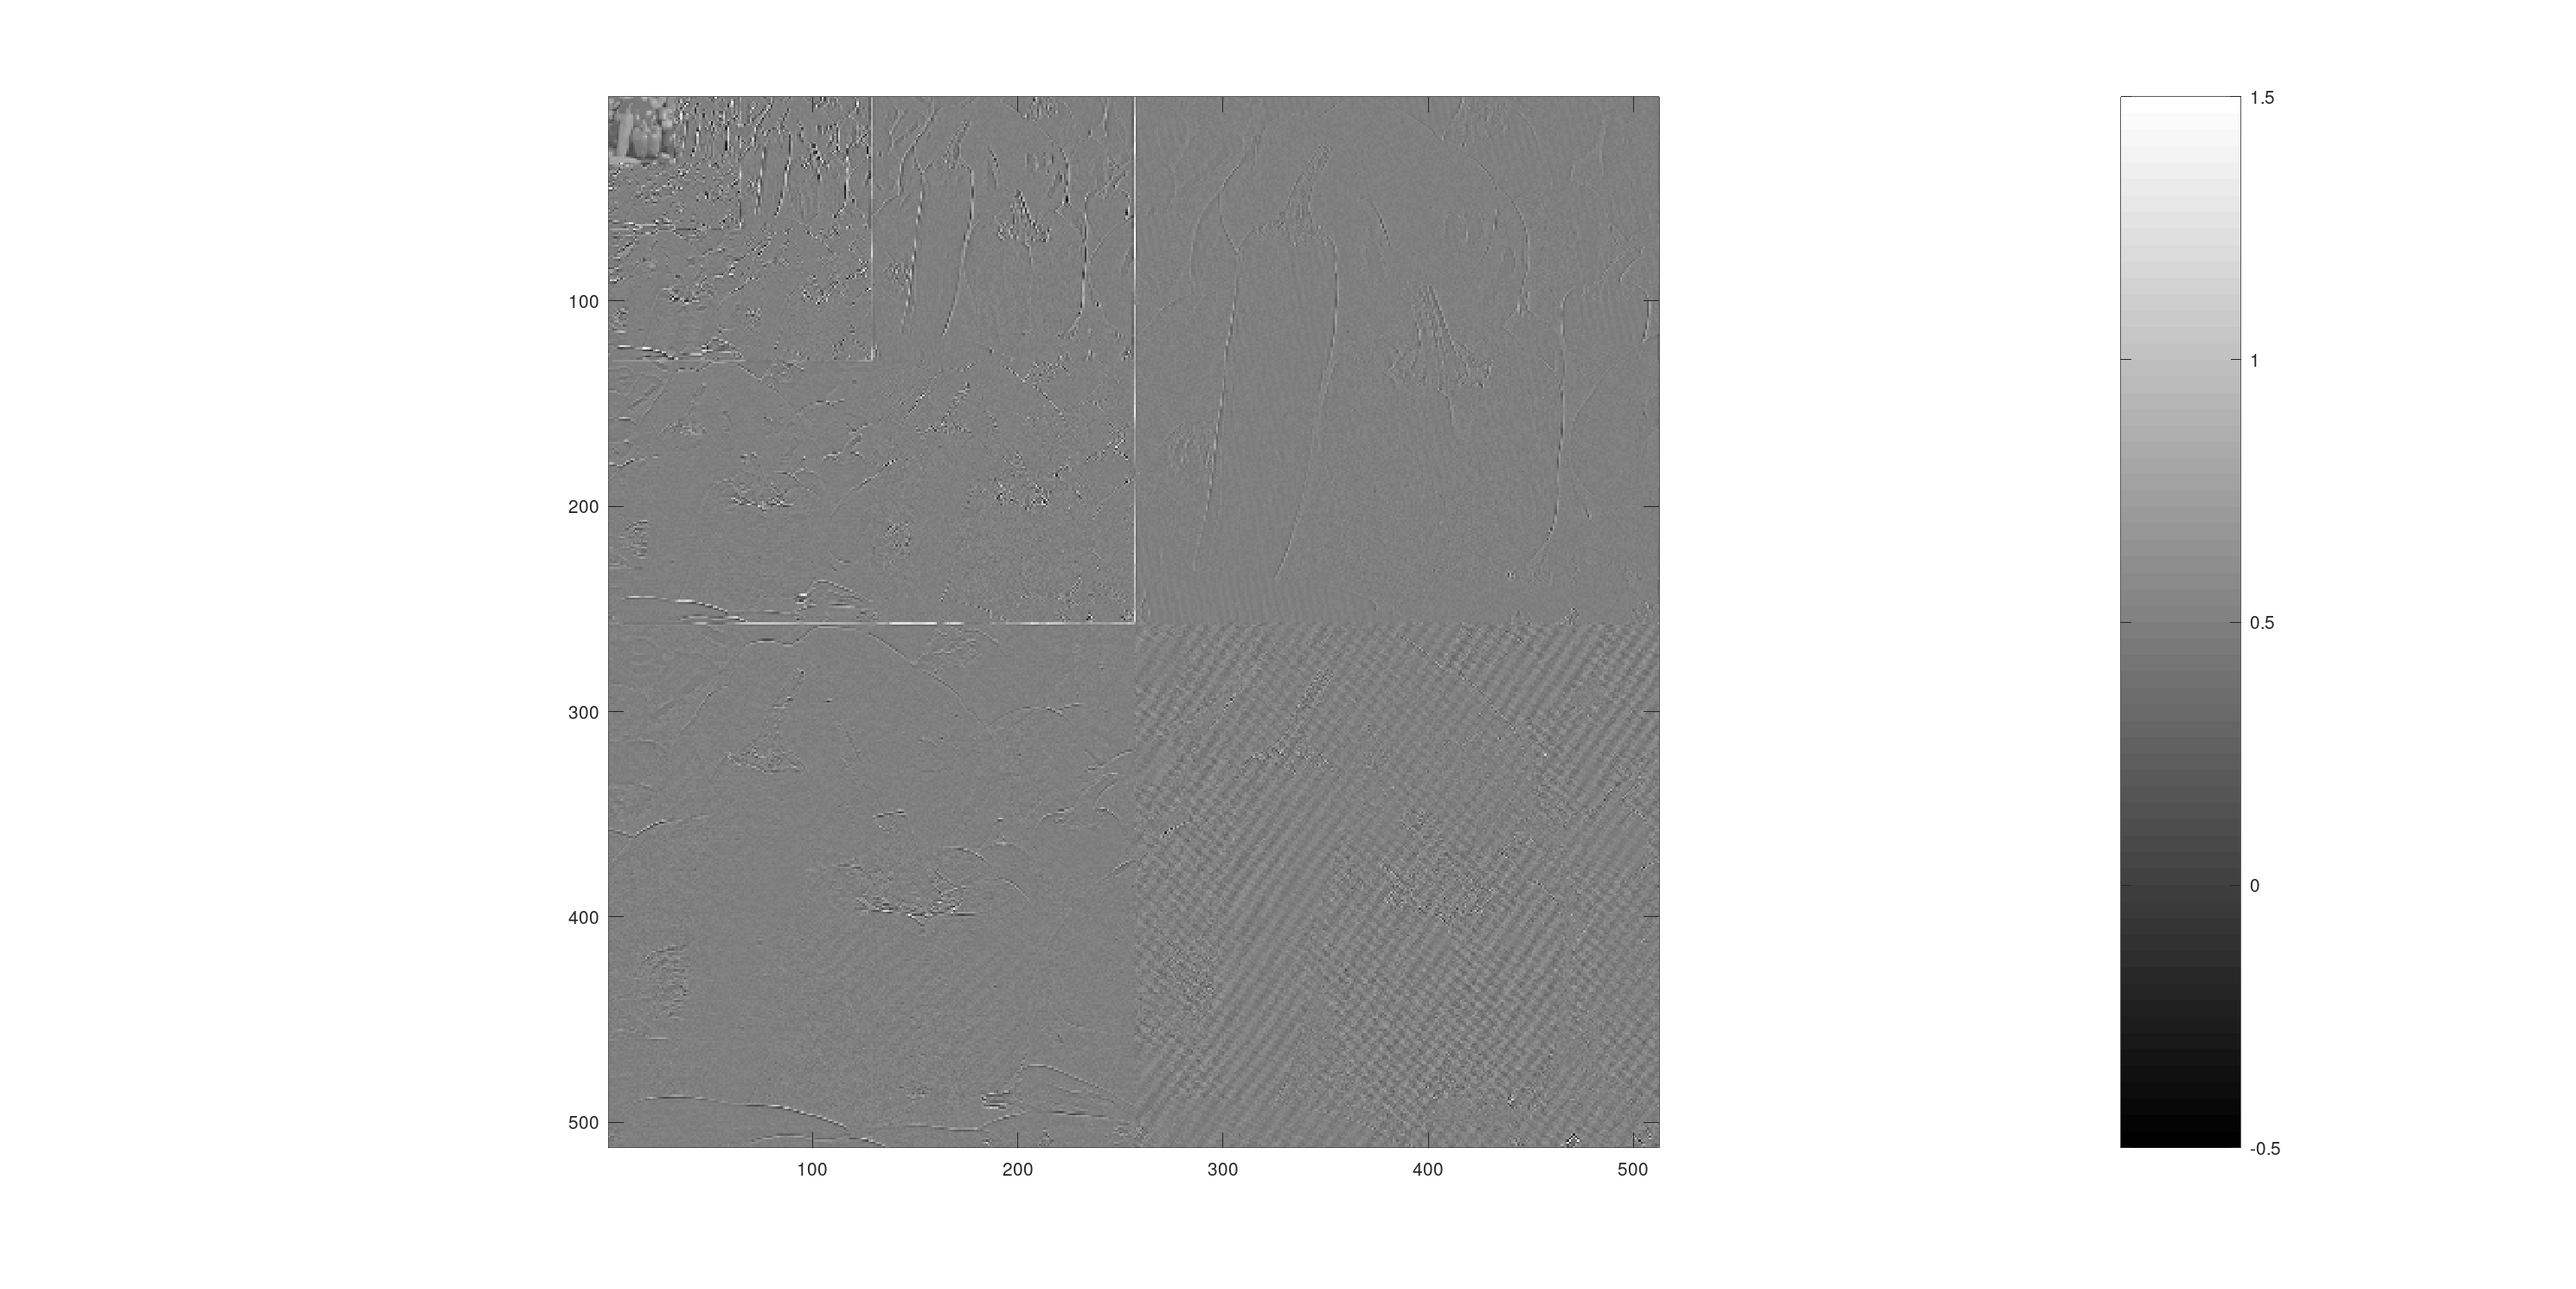
\includegraphics[width=\textwidth]{ex3_2}
                    \centering
                \end{figure}
            }

        \item{Représentons l'histogramme des coefficients et traçons les par
                ordre décroissant en valeur absolue :

                \begin{figure}[H]
                    \caption{Histogramme}
                    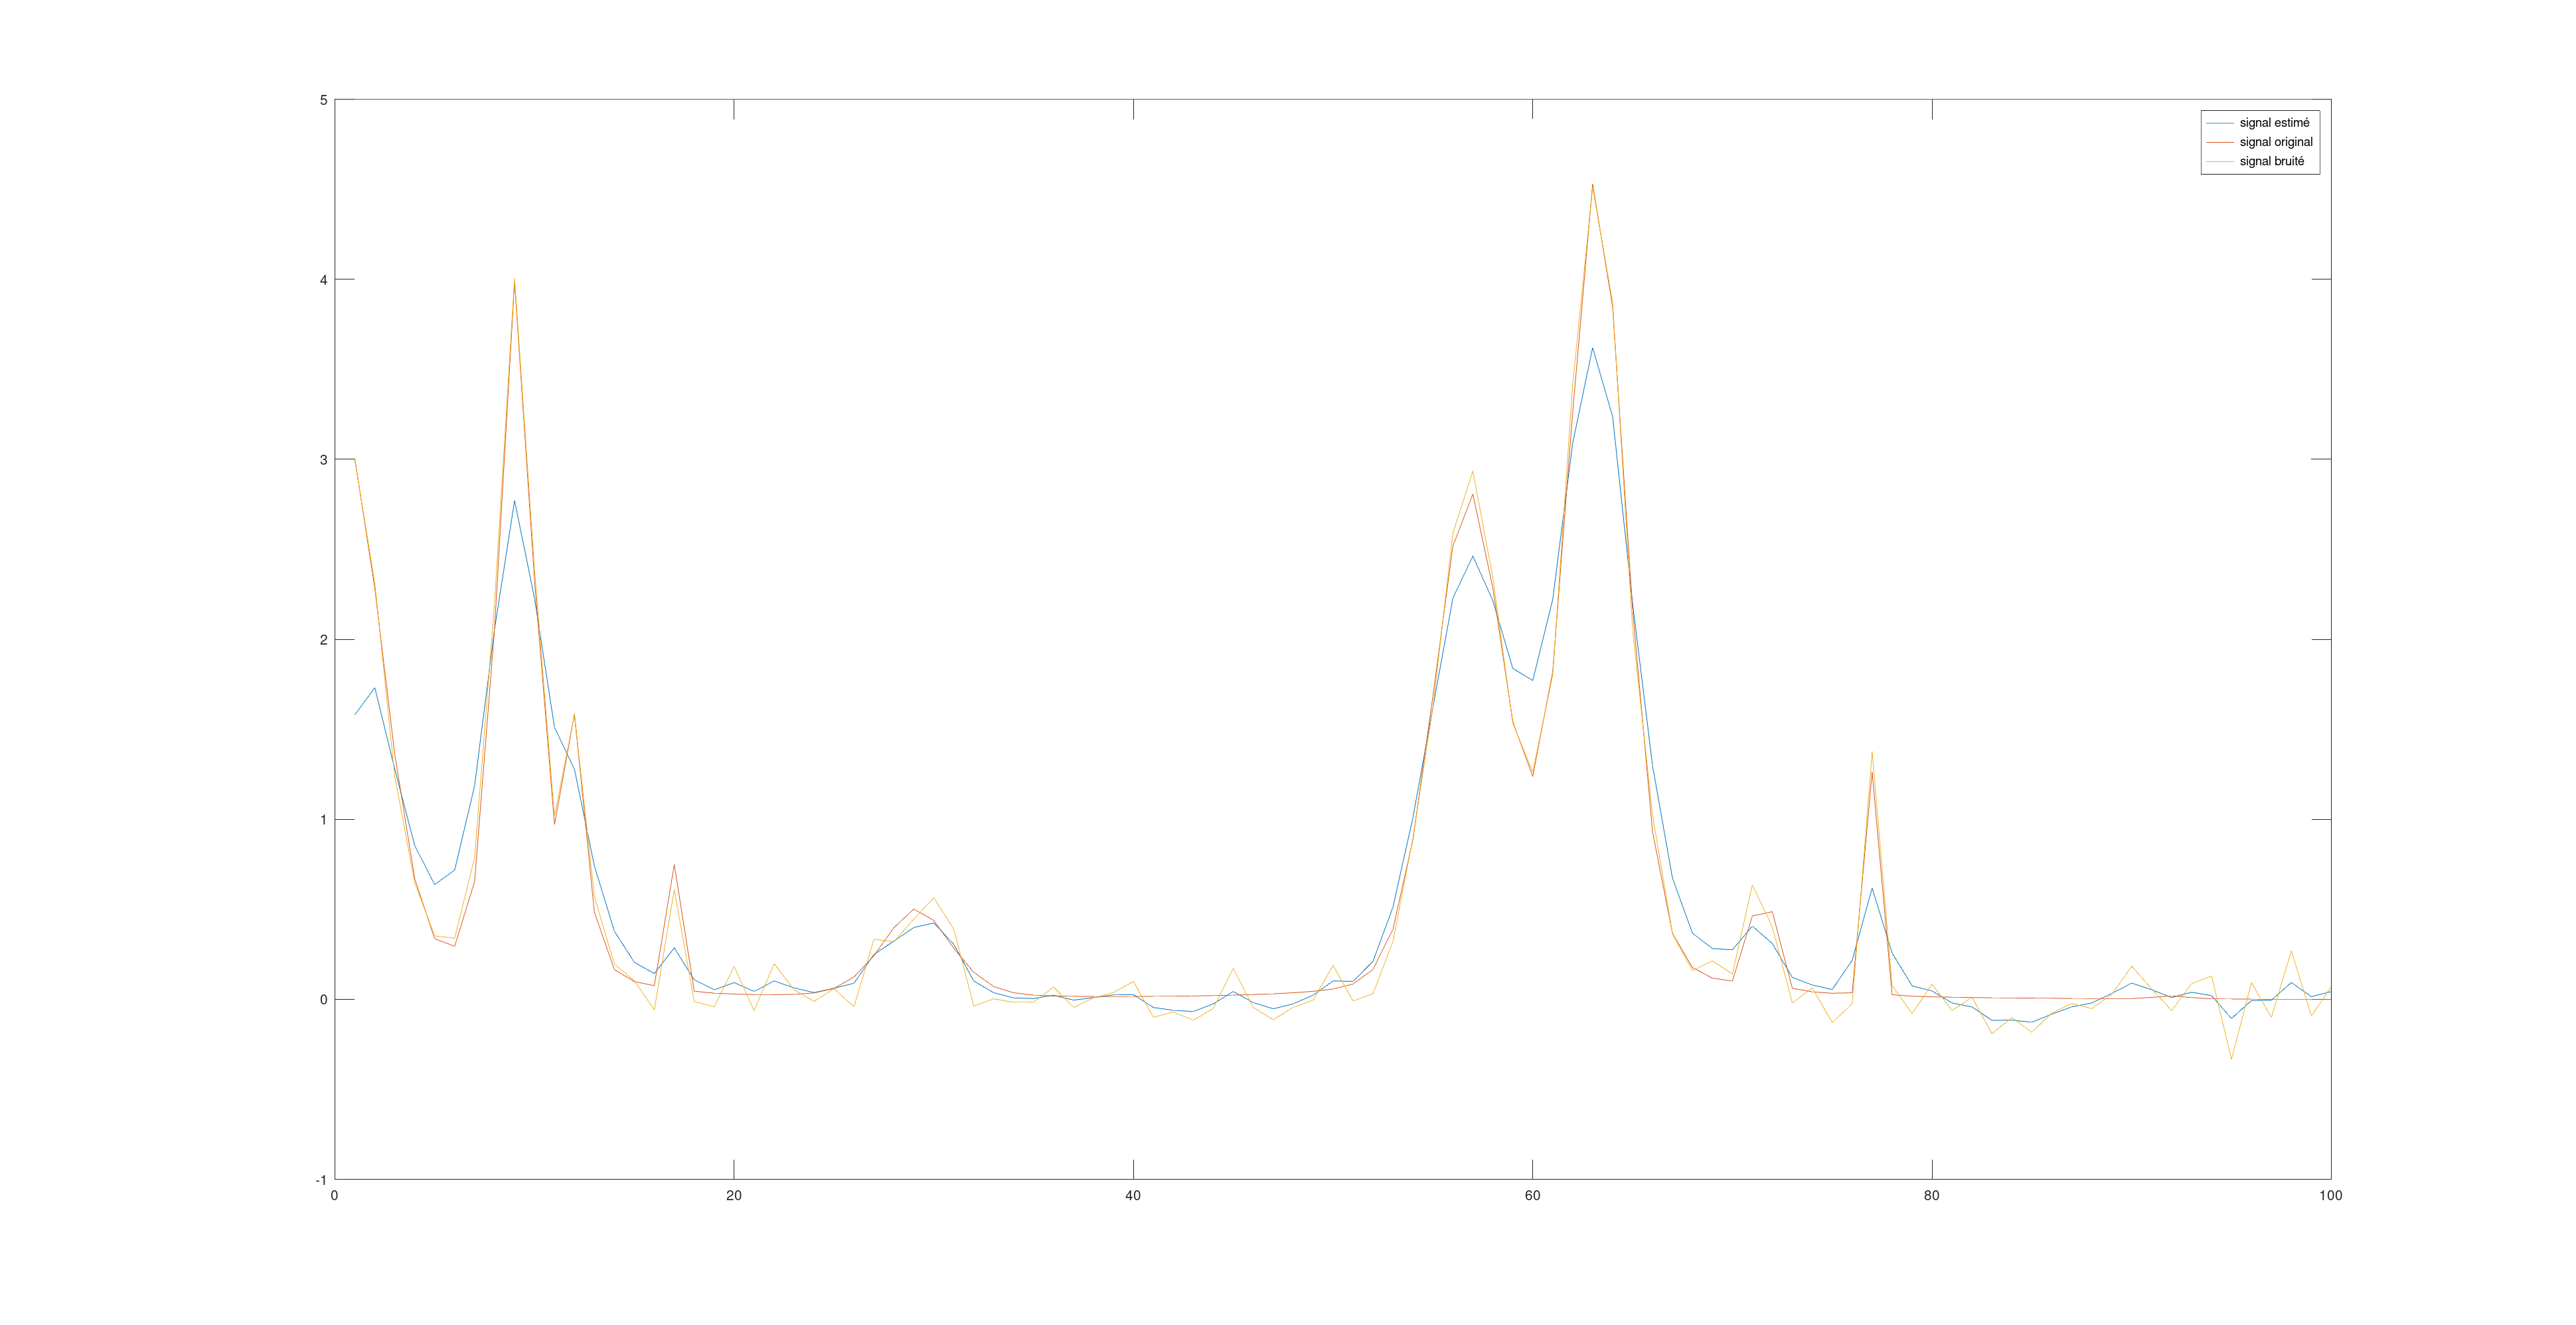
\includegraphics[width=\textwidth]{ex3_3}
                    \centering
                \end{figure}

                \begin{figure}[H]
                    \caption{coefficients (ordre décroissant)}
                    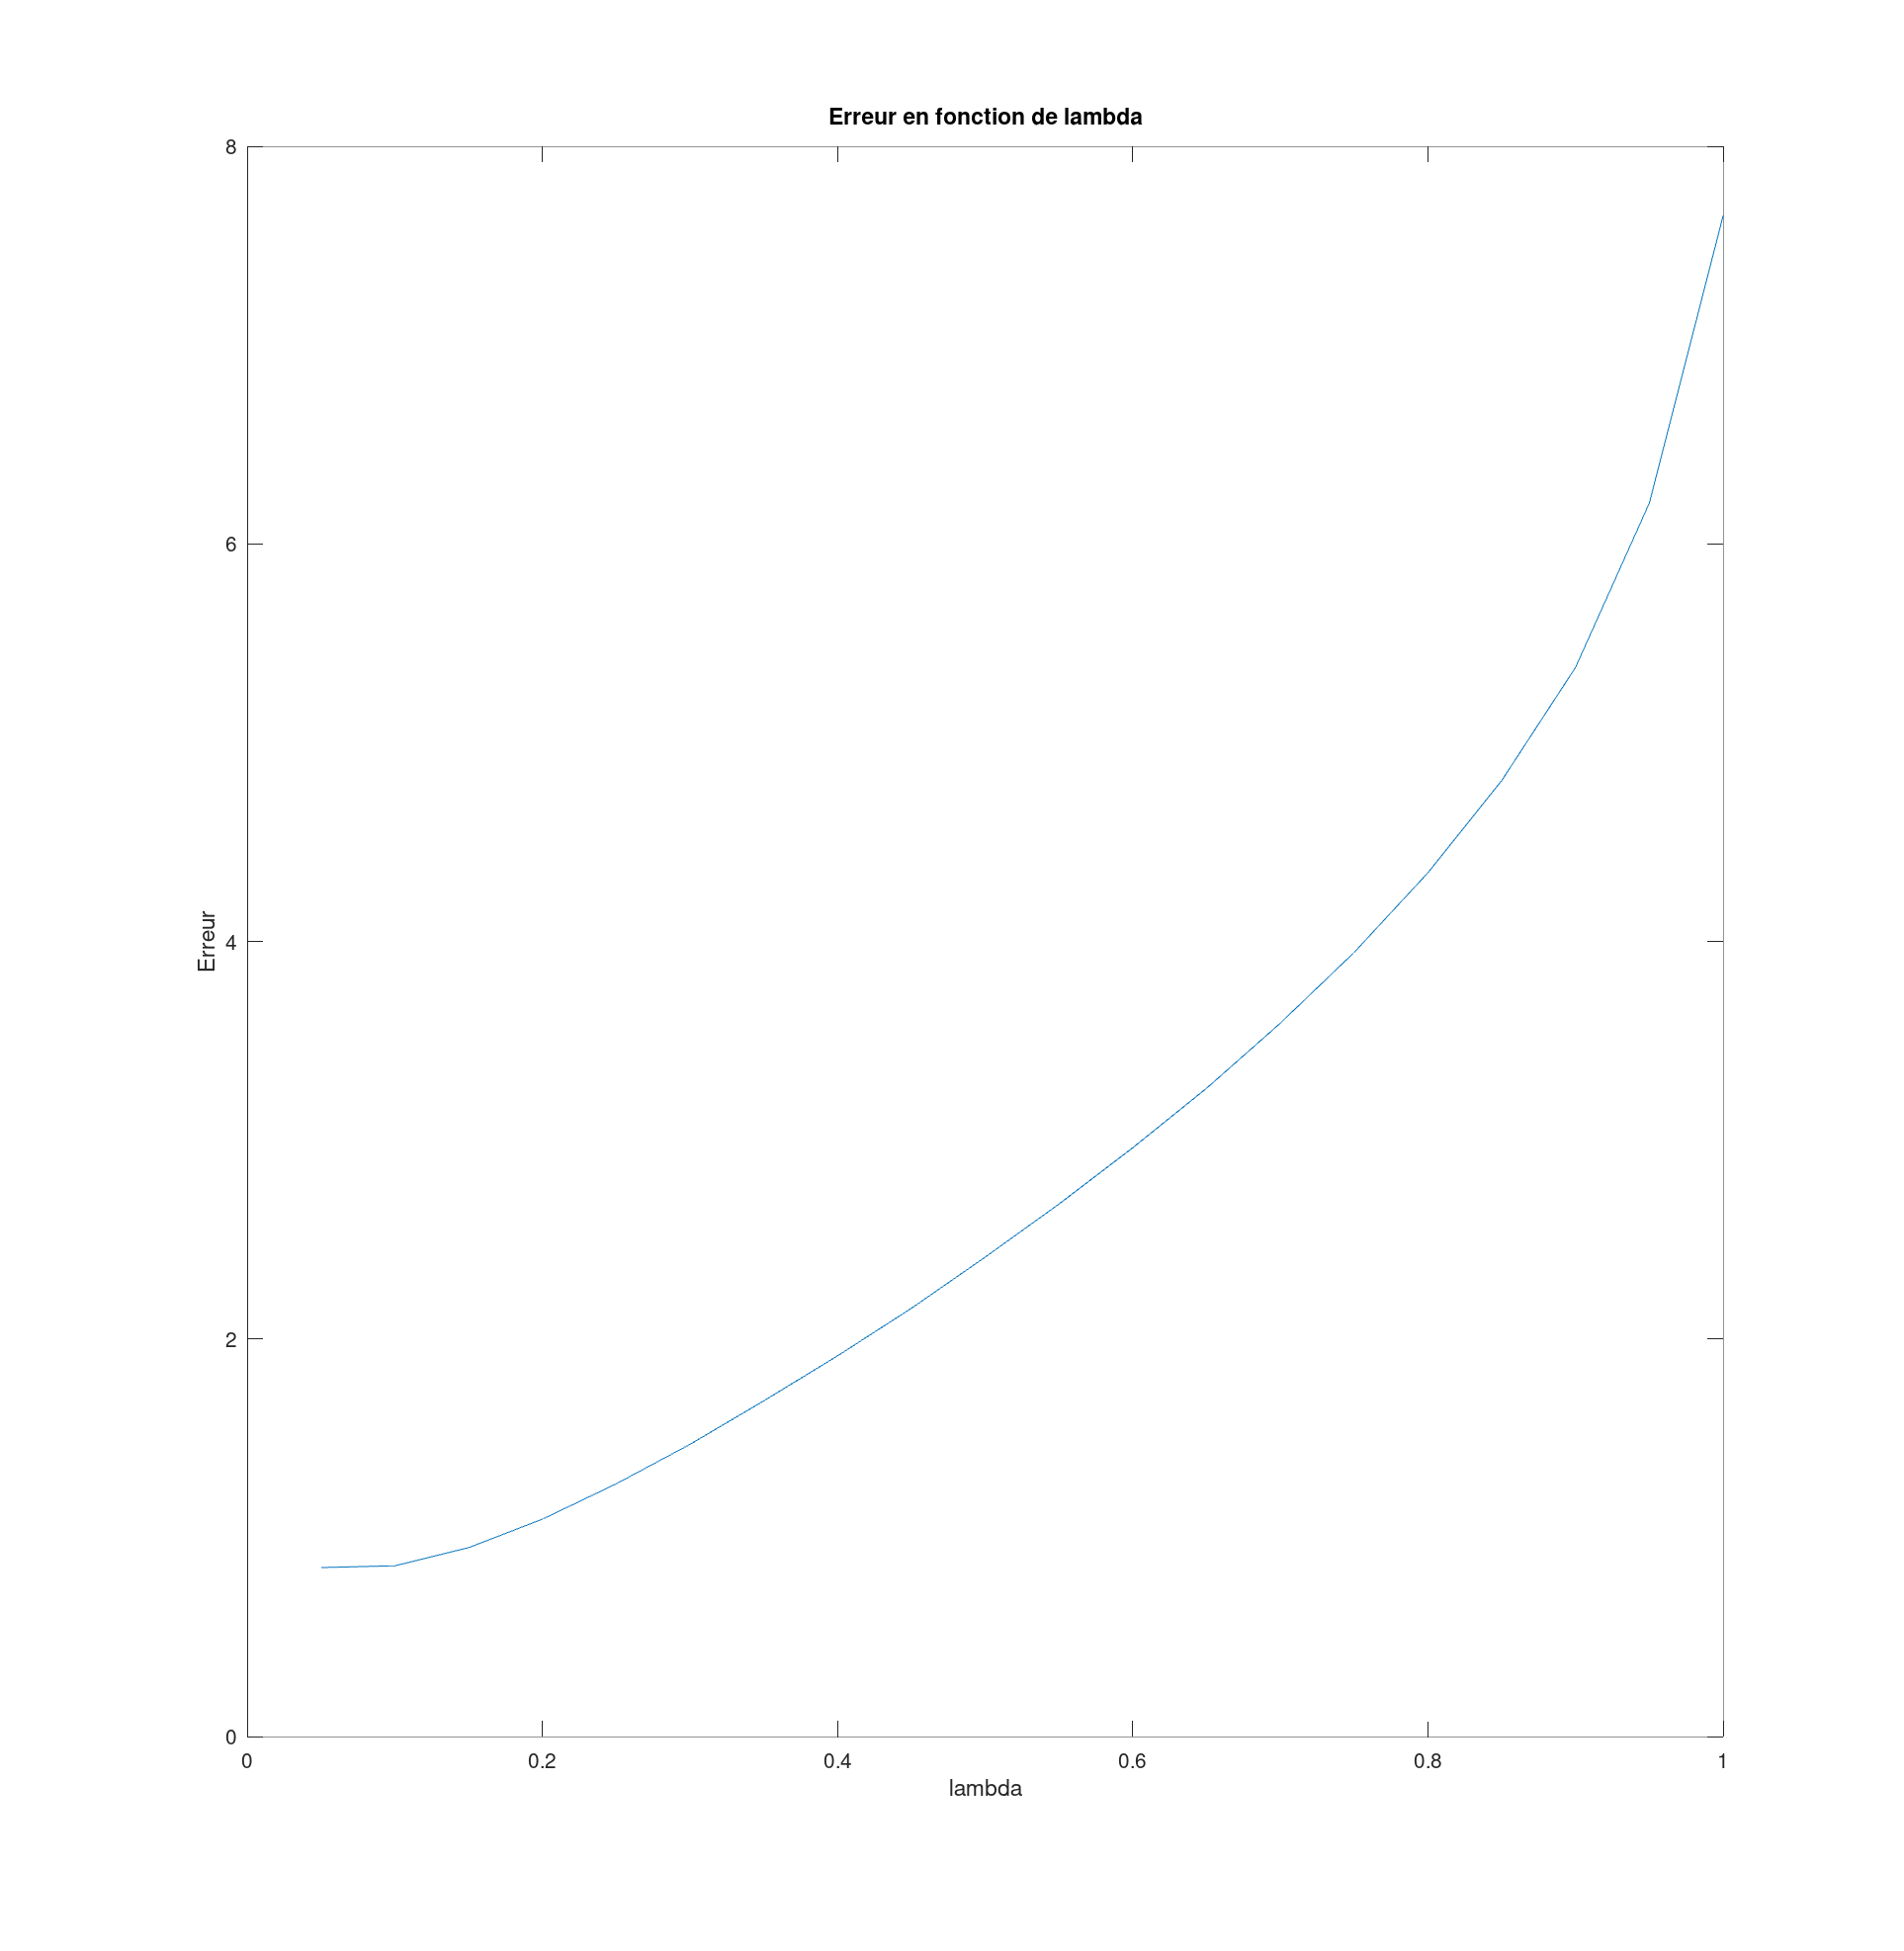
\includegraphics[width=\textwidth]{ex3_4}
                    \centering
                \end{figure}

            }

        \item{{La procédure de compression consiste en la reconstruction de l'image à partir de sa DWT
                seuillée. On se donne un $\tau$ et on ne conserve que les $\tau \%$ coefficients
                les plus grands.
            }

        \item{Visualisions l'image reconstruite pour $\tau \in \{1,5,20\}$.

                \begin{figure}[H]
                    \caption{Résultats pour $\tau = 1\%$}
                    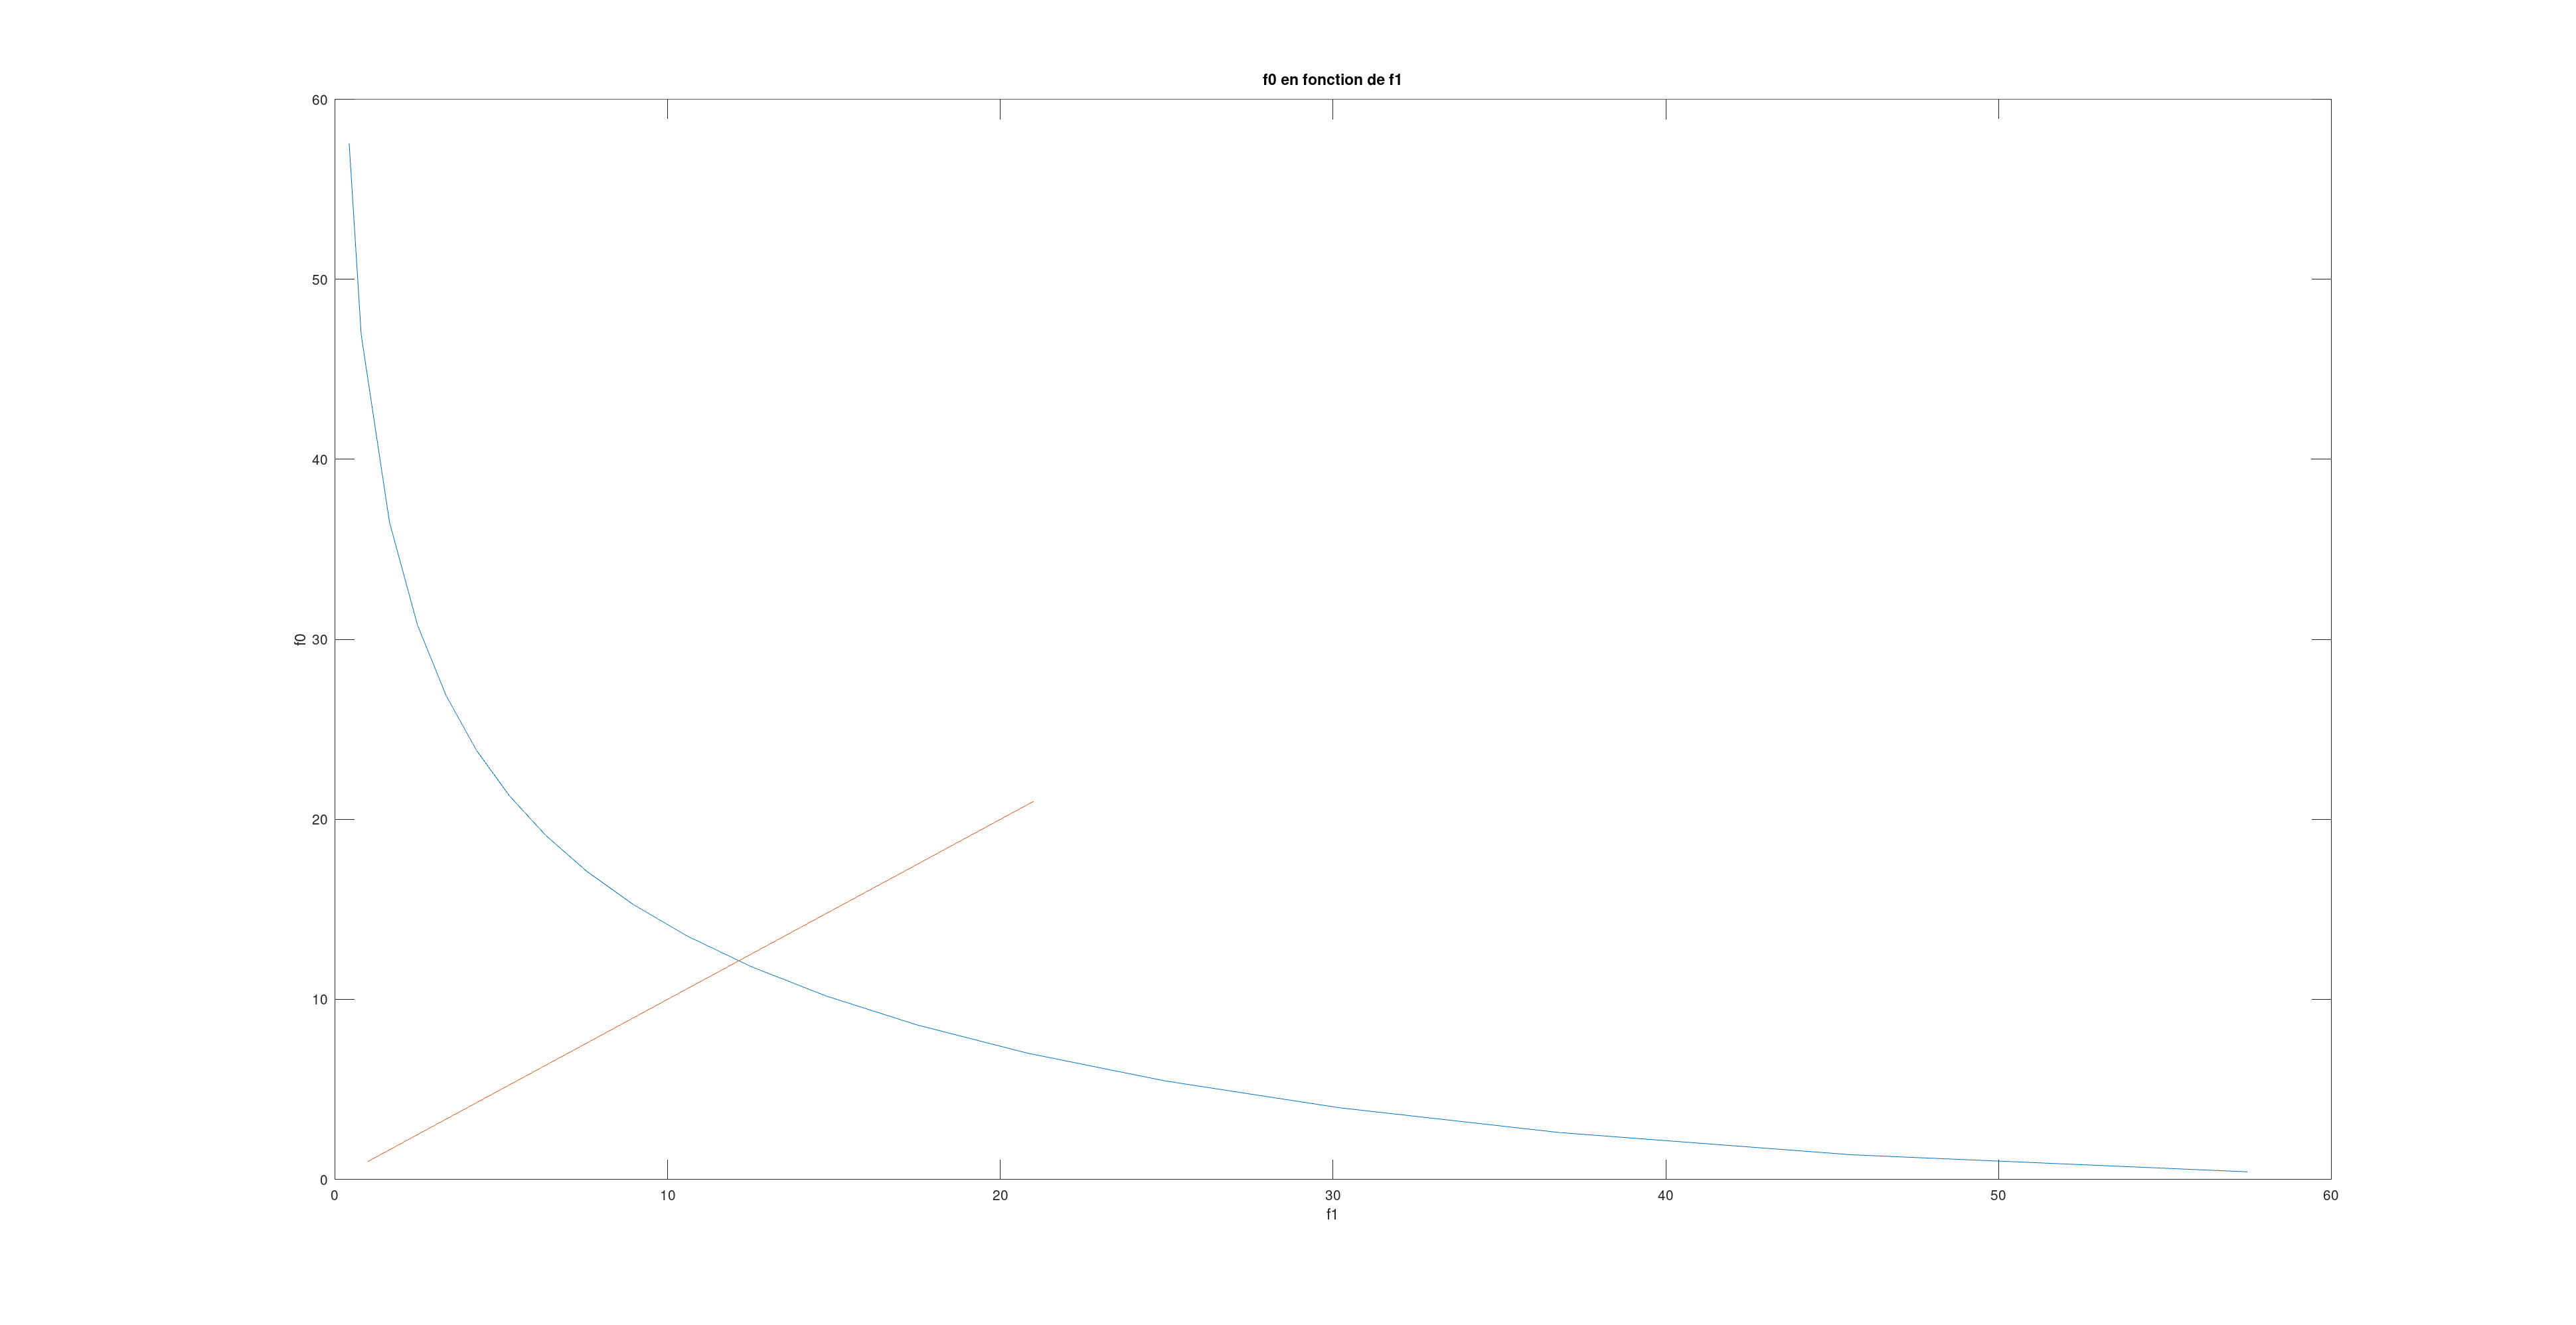
\includegraphics[width=\textwidth]{ex3_5}
                    \centering
                \end{figure}

                \begin{figure}[H]
                    \caption{Résultats pour $\tau = 5\%$}
                    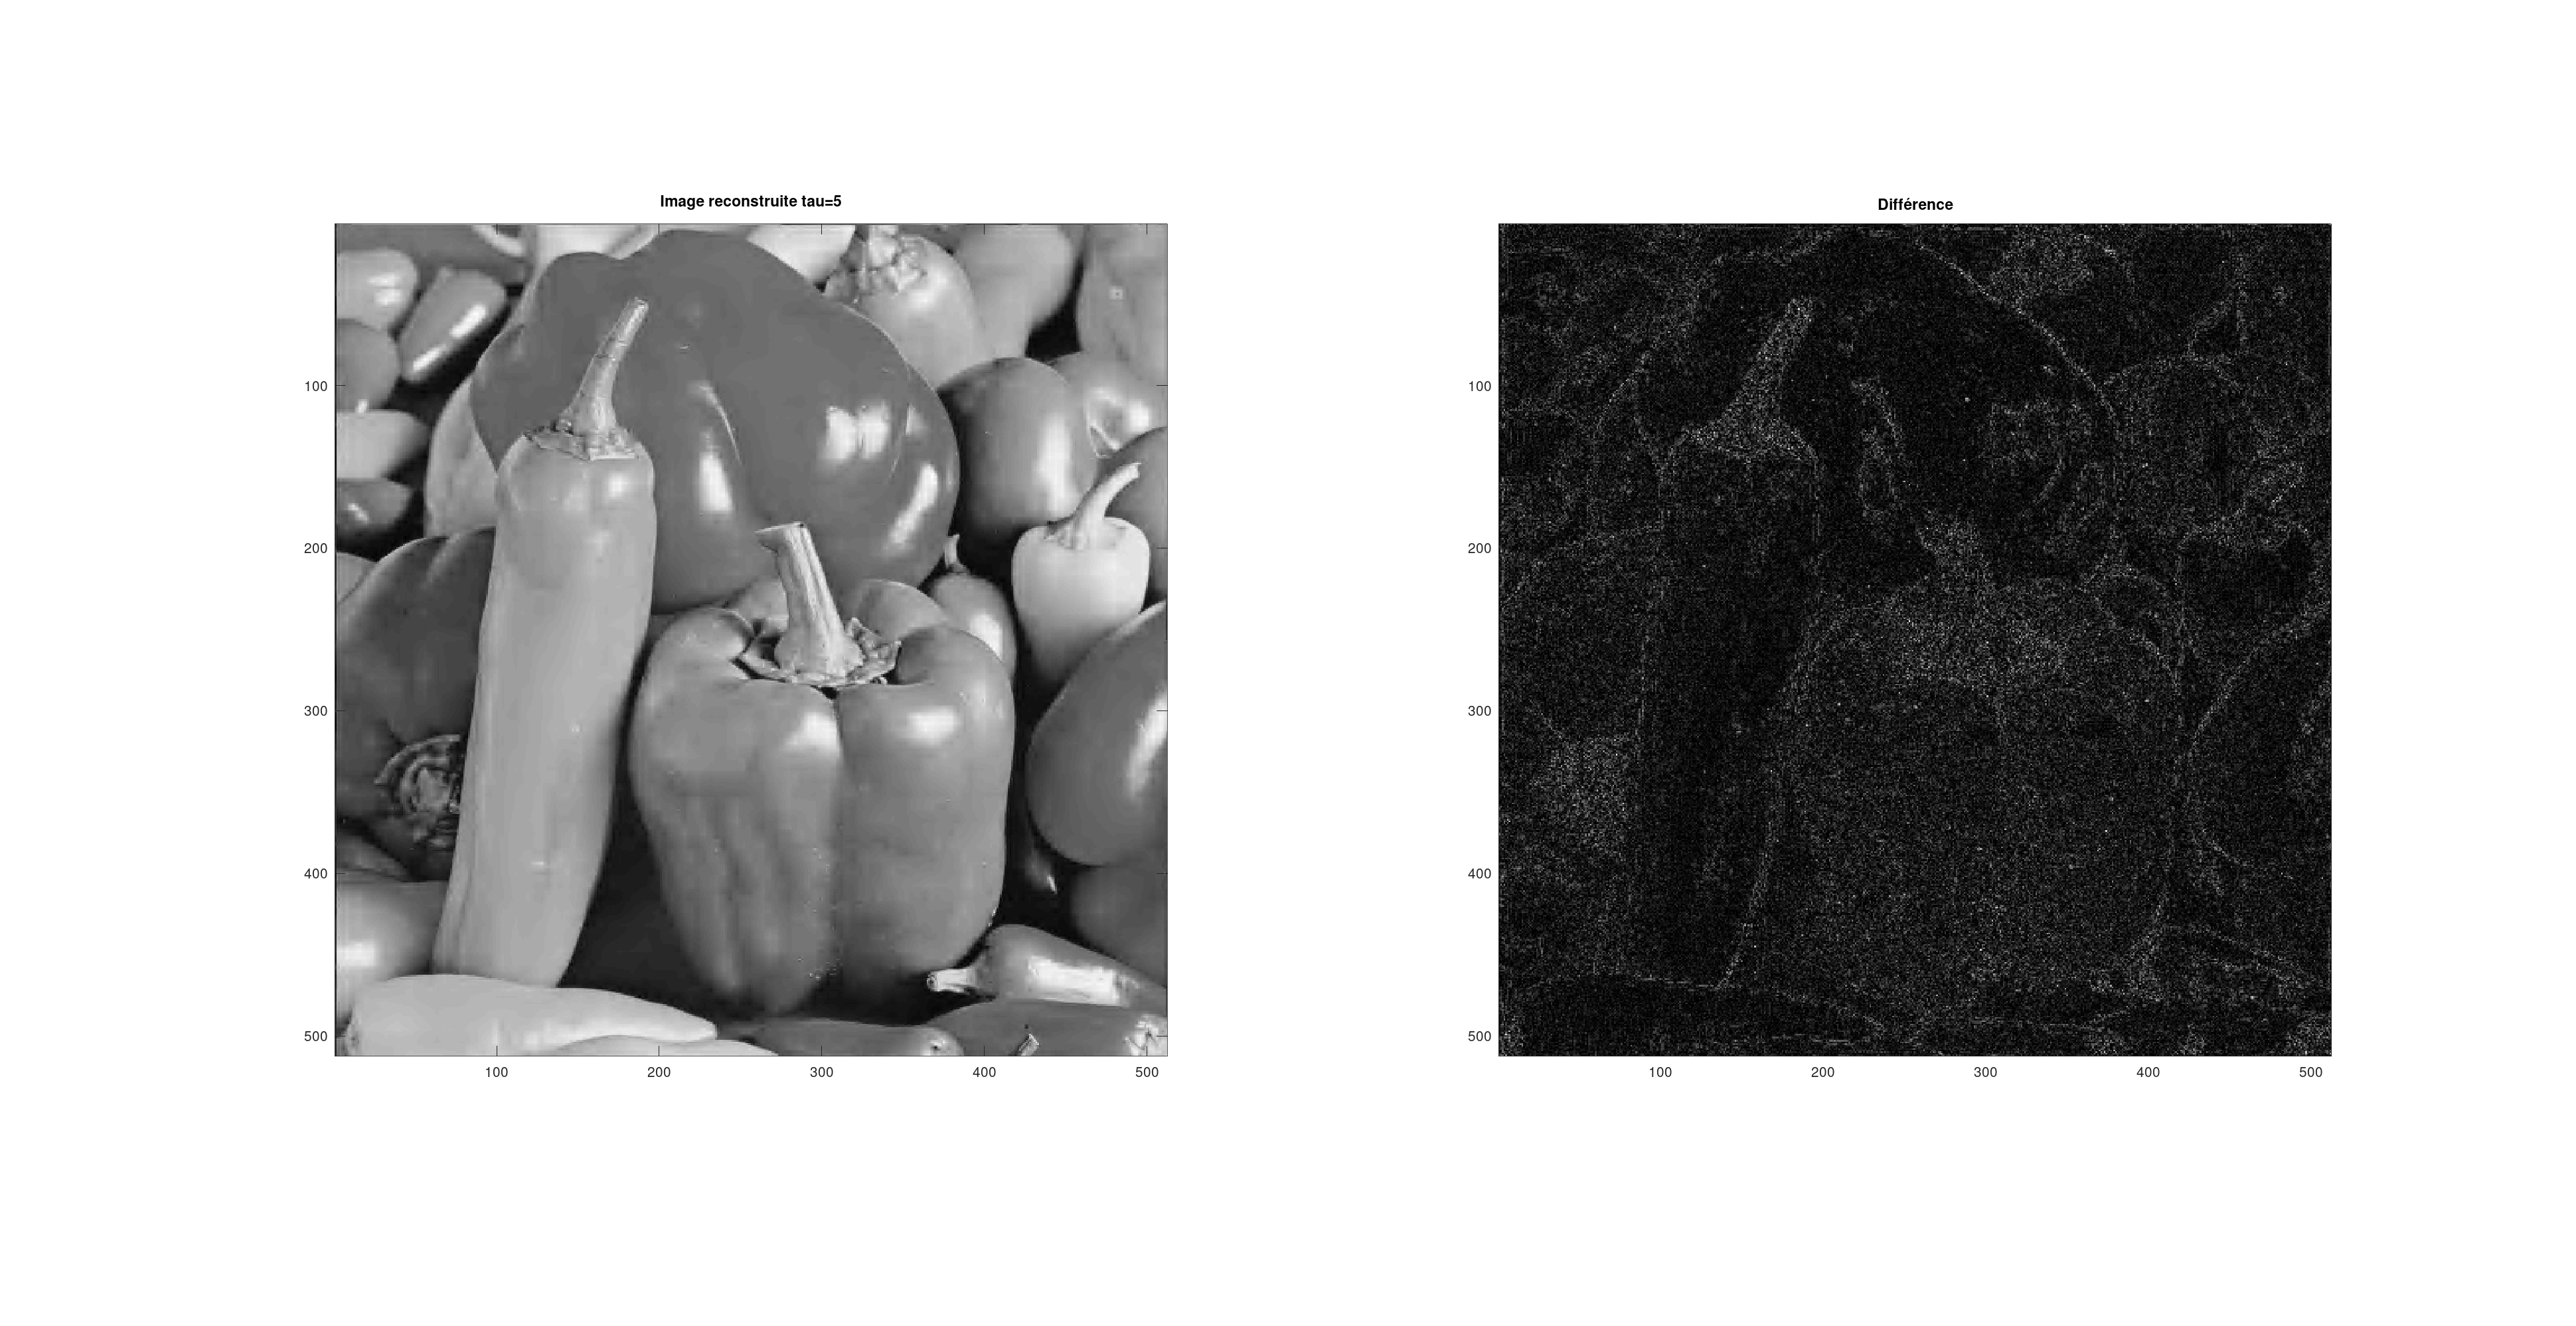
\includegraphics[width=\textwidth]{ex3_6}
                    \centering
                \end{figure}

                \begin{figure}[H]
                    \caption{Résultats pour $\tau = 20\%$}
                    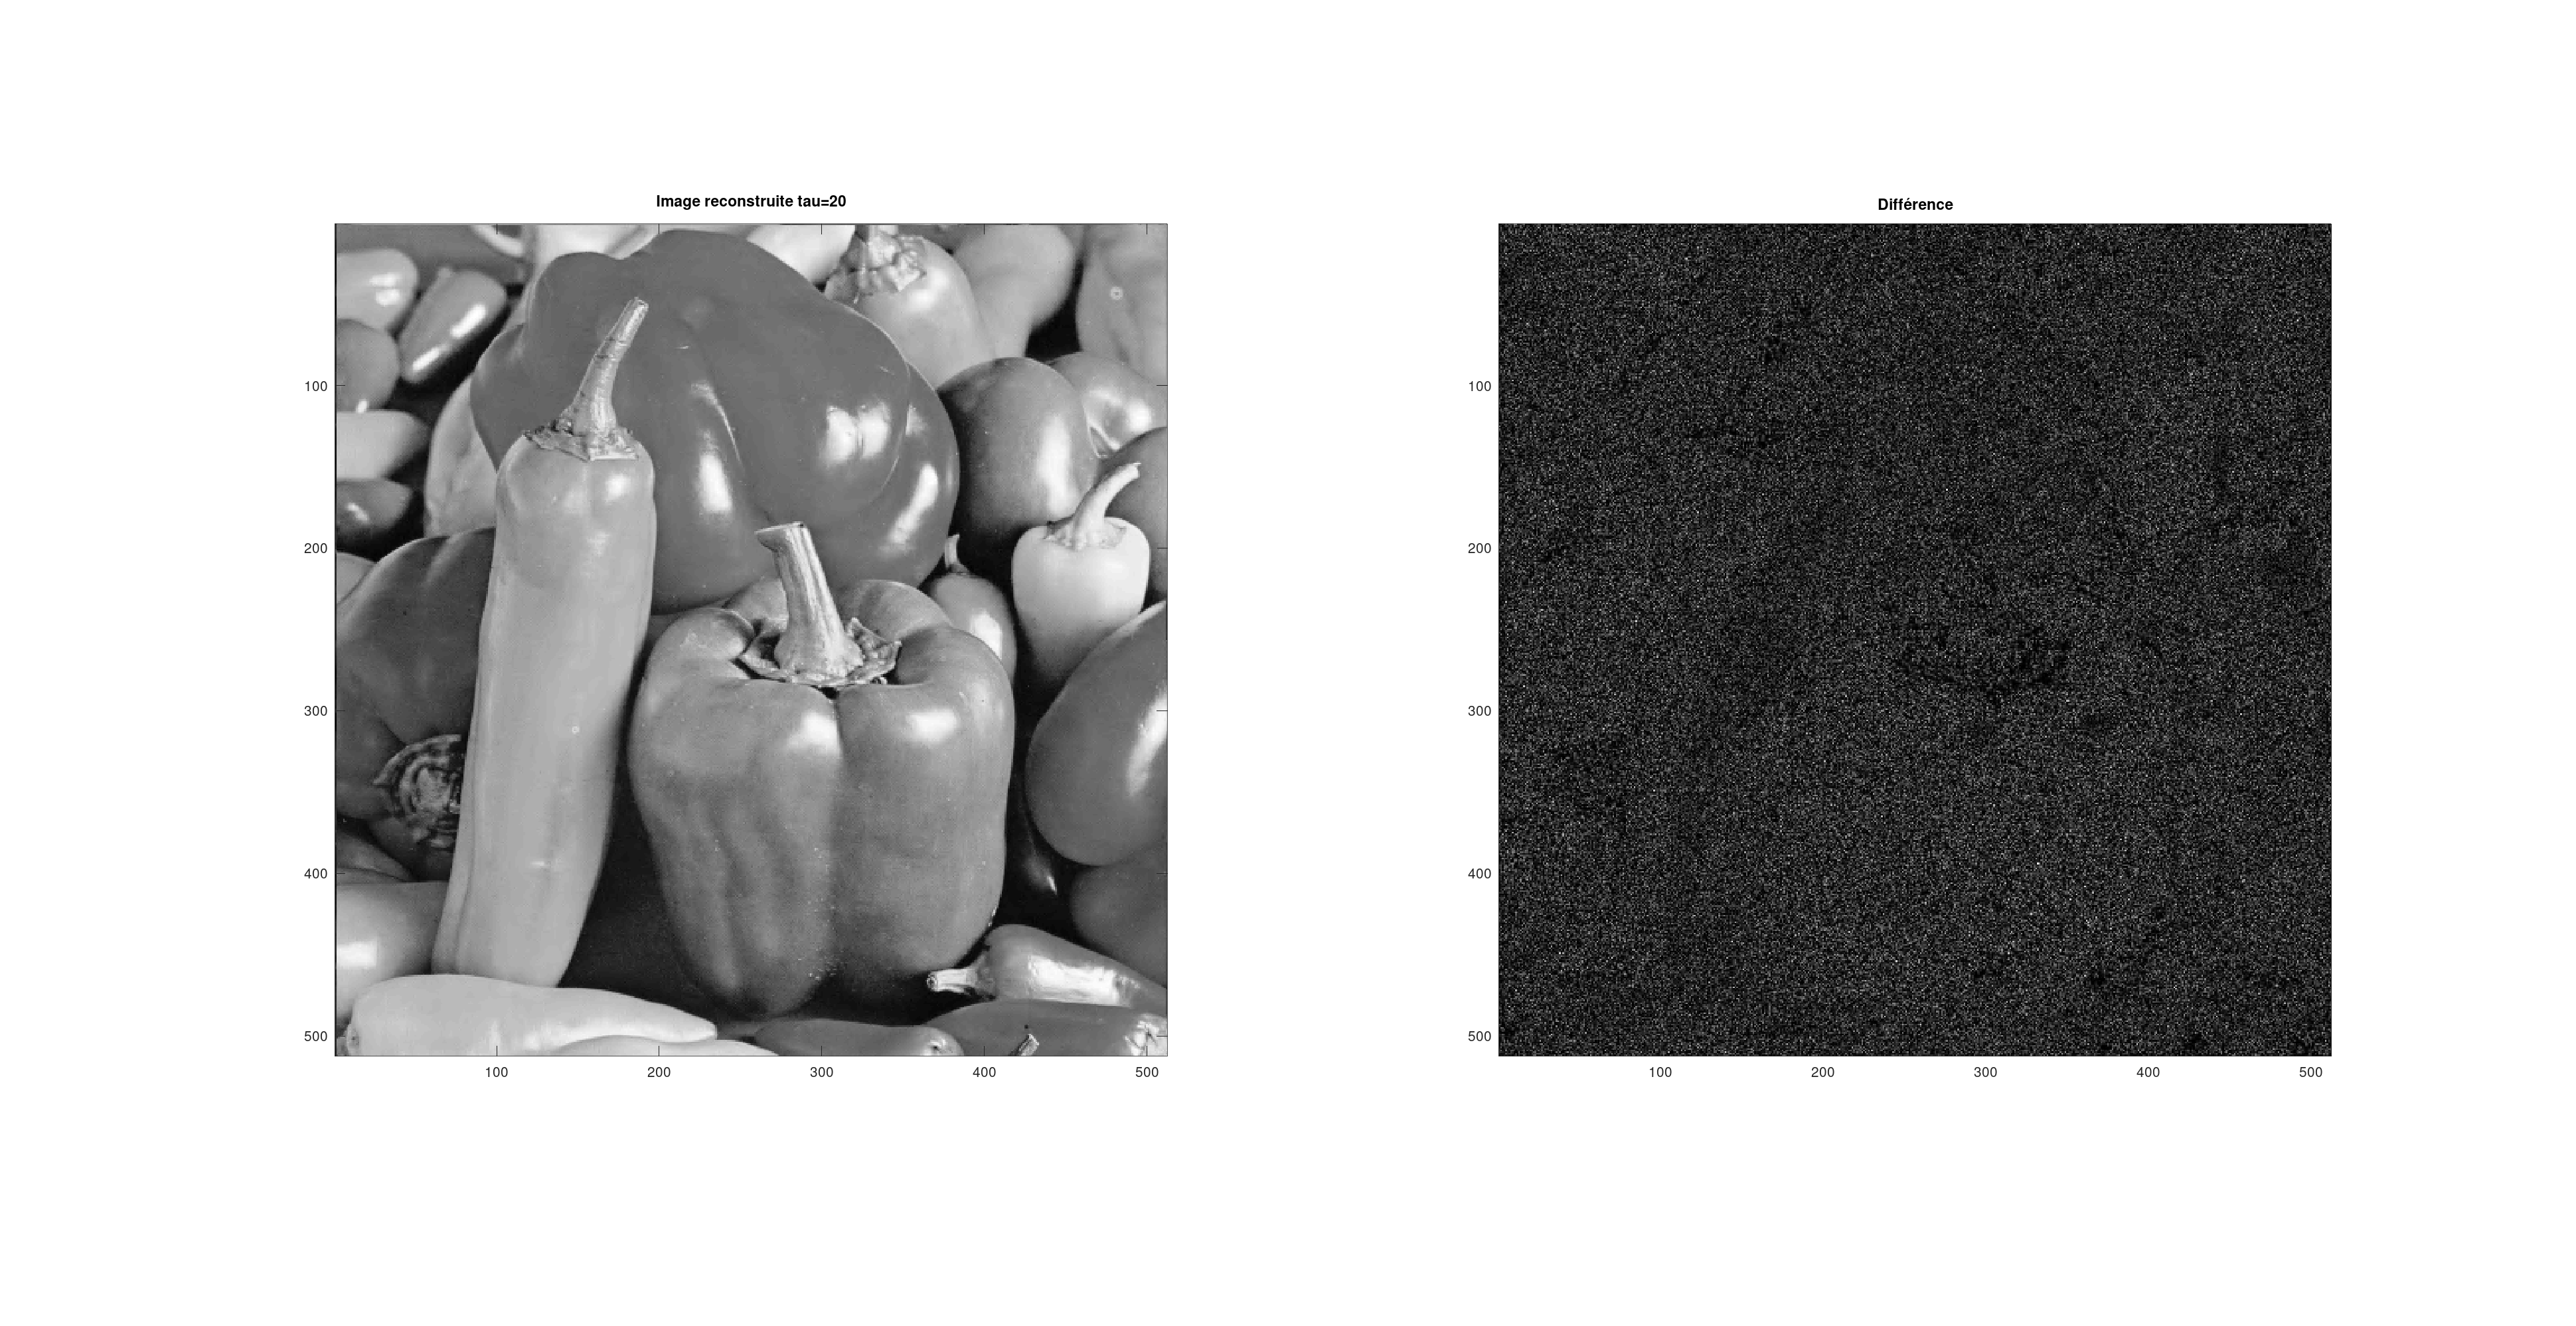
\includegraphics[width=\textwidth]{ex3_7}
                    \centering
                \end{figure}
            }

        \end{enumerate}

        \section*{Conclusion}

\end{enumerate}

\end{document}
